% ---------------------------------------------------------------------------
% Author guideline and sample document for EG publication using LaTeX2e input
% D.Fellner, v1.13, Jul 31, 2008

\documentclass{egpubl}
\usepackage{eurovis2016}

% --- for  Annual CONFERENCE
% \ConferenceSubmission   % uncomment for Conference submission
% \ConferencePaper        % uncomment for (final) Conference Paper
% \STAR                   % uncomment for STAR contribution
% \Tutorial               % uncomment for Tutorial contribution
% \ShortPresentation      % uncomment for (final) Short Conference Presentation
% \Areas                  % uncomment for Areas contribution
% \MedicalPrize           % uncomment for Medical Prize contribution
% \Education              % uncomment for Education contribution
%
% --- for  CGF Journal
% \JournalSubmission    % uncomment for submission to Computer Graphics Forum
% \JournalPaper         % uncomment for final version of Journal Paper
%
% --- for  CGF Journal: special issue
% \SpecialIssueSubmission    % uncomment for submission to Computer Graphics Forum, special issue
\SpecialIssuePaper         % uncomment for final version of Journal Paper, special issue
%
% --- for  EG Workshop Proceedings
% \WsSubmission    % uncomment for submission to EG Workshop
% \WsPaper         % uncomment for final version of EG Workshop contribution
%
 \electronicVersion % can be used both for the printed and electronic version

% !! *please* don't change anything above
% !! unless you REALLY know what you are doing
% ------------------------------------------------------------------------

% for including postscript figures
% mind: package option 'draft' will replace PS figure by a filname within a frame
\ifpdf \usepackage[pdftex]{graphicx} \pdfcompresslevel=9
\else \usepackage[dvips]{graphicx} \fi

\PrintedOrElectronic

% prepare for electronic version of your document
\usepackage{t1enc,dfadobe}

\usepackage{egweblnk}
\usepackage{cite}

\usepackage{subfig}
\usepackage{epstopdf}


% For backwards compatibility to old LaTeX type font selection.
% Uncomment if your document adheres to LaTeX2e recommendations.
% \let\rm=\rmfamily    \let\sf=\sffamily    \let\tt=\ttfamily
% \let\it=\itshape     \let\sl=\slshape     \let\sc=\scshape
% \let\bf=\bfseries

% end of prologue

%\hyphenation{cellPack}

% ---------------------------------------------------------------------
% EG author guidelines plus sample file for EG publication using LaTeX2e input
% D.Fellner, v1.17, Sep 23, 2010


\title[Visibility Equalizers]%
      {Visibility Equalizers for Molecular Visualization}

% for anonymous conference submission please enter your SUBMISSION ID
% instead of the author's name (and leave the affiliation blank) !!
\author[M. Le Muzic et al.]
       {M. Le Muzic\thanks{mathieu@cg.tuwien.ac.at}$^{1}$,
        P. Mindek\thanks{mindek@cg.tuwien.ac.at}$^{1}$,
        J. Sorger\thanks{sorger@cg.tuwien.ac.at}$^{1,2}$,
        L. Autin\thanks{ludovic.autin@gmail.com}$^{3}$,
        and I. Viola\thanks{viola@cg.tuwien.ac.at}$^{1}$        
        \\
% For Computer Graphics Forum: Please use the abbreviation of your first name.
         $^1$TU Wien, Austria \\
         $^2$VRVis Research Company, Austria \\
        $^3$ The Scripps Research Institute, La Jolla, California, USA
%             with different affiliations
       }

% ------------------------------------------------------------------------

% if the Editors-in-Chief have given you the data, you may uncomment
% the following five lines and insert it here
%
% \volume{27}   % the volume in which the issue will be published;
% \issue{1}     % the issue number of the publication
% \pStartPage{1}      % set starting page


%-------------------------------------------------------------------------
\begin{document}

% \teaser{
%  
\includegraphics[width=\linewidth]{eg_new}
%  \centering
%   \caption{New EG Logo}
% \label{fig:teaser}
% }

\maketitle

\begin{abstract}
In scientific illustration and visualization, cutaway views are often employed as an effective technique for occlusion management in densely packed scenes.
We propose a novel data-centric method for authoring cutaway illustrations of mesoscopic biological models.
In contrast to the existing cutaway algorithms, we take advantage of the specific nature of the biological models. These models consist of thousands of instances that are distributed across a comparably smaller number of different molecular types.
Our method constitutes a two stage process.
In the first step, culling objects are placed in the scene, creating a cutaway visualization of the model.
During this process, histograms inform the user about the instance visibility distribution of each individual molecular type in the scene.
In the second step, the visibility of each molecular type is fine-tuned through these histograms, which at this point act as interactive visibility equalizers. %The visibility equalizers give illustrators precise control over how much percent of each type of molecule should be visible in front of the cutting object. Thus enabling them to quickly and efficiently create visualizations of biological models that provide insights  which would have taken them to manually recreate.
The technique has been evaluated by domain experts in scientific illustration.




%In molecular biology and similar fields, knowledge transfer is commonly carried out through schematic illustrations.
%Traditionally, illustrations of biological processes on the molecular level have been created by manual hand drawing.
%Nowadays, complex models of various biochemical structures and micro-organisms exist.
%These models can be utilized in creating computer-generated biological illustrations through various molecular-visualization algorithms.
%When using such algorithms, it is beneficial for illustrators to be able to apply techniques common in traditional illustration, such as cutaway views.
%In this paper, we propose a method for enhancing real-time molecular-visualization algorithms with the capability to apply cutaway views.
%In contrast with existing cutaway algorithms, we take advantage of the specific nature of the biochemical models, which consists of multiple instances of a limited number of different molecular types.
%Our approach to cutaway views allows the illustrators to reintroduce some of the removed instances into the scene to communicate the presence of the given molecular type, yet maintaining the visibility of the internal structures of the model.
%This process is enabled through a novel interaction method for controlling the visibility in the instance-based scene. We refer to this method as visibility equaliser.


%In this paper, we propose a method for enhancing real-time molecular-visualization algorithms with the capability to display cutaway views.
%Such an option is beneficial to biological illustrators, since the technique of cutaway display is ubiquitously applied in traditional illustration.
%In contrast with existing algorithms for creating cutaway views, we take advantage of the specific nature of the biochemical models, which consist of multiple instances of the limited number of different molecular types.
%We are able to create comprehensible illustrations of complex models by reintroducing some of these instances in the cutaway parts of the rendered illustration.
%The main contribution of this paper is an interaction mechanism which allows the illustrators to precisely control the amount of instances of different molecular types in the illustration, while maintaining the desired information value.

\begin{classification} % according to http://www.acm.org/class/1998/
\CCScat{Computer Graphics}{I.3.3}{Picture/Image Generation}{Viewing algorithms}
\end{classification}

\end{abstract}




%-------------------------------------------------------------------------
\section{Introduction}

Biology is an emerging field where the state of the current knowledge changes extremely quickly.
New discoveries have to be communicated to a large variety of audiences.
Since these discoveries often happen on the microscopic level and they are not directly observable in sufficient detail, illustration is the only way how to communicate them.

Traditional pipeline of the scientific illustrators starts with the collection of data and knowledge gathering.
Afterwards, they make sketches, in which specific regions of the illustrated objects are uncovered.
For this, occlusion management techniques are necessary.
Oftentimes, \emph{cutaway views} are employed, where specific parts of the scene are removed form the illustration, so that internal structures become visible.
When new knowledge is discovered, the conceptual layout of the illustration might break down and the whole process has to start from the beginning.
Therefore, the duration of this process counts in months or even years.

With the rapid changes to the knowledge in the field of biology, it is necessary to adapt the traditional illustration pipeline so that the new data can be easily plugged in and the resulting illustrations can be updated accordingly in a very short time period.
Virtual models of cells and other mesoscale molecular structures can be utilized for this purposes.
These models can be created with tools such as \emph{cellPack} \cite{cellpack} and the knowledge from the field of integrative structural biology.
The models consist of multiple instances of several molecular types.
The instances are densely packed within predefined compartments according to the biology knowledge.

The mesoscale biological models represent the geometry of microorganisms, cells, or even viruses at atomic resolution.
However, simply displaying such models does not guarantee an adequate view of internal structures, which are often necessary to communicate through an illustration.
This is due to the high density of the molecular instances present in the models.
To solve this problem, visualization techniques need to be developed which reproduce the occlusion management methods used in traditional illustration.

Currently, occlusion management in virtual models is carried out by placing culling objects in the scene, which remove specified parts of the displayed model.
During this process, the illustrator does not have a good overview of what instances have been already removed, and which molecular types are still sufficiently represented in the scene.
The illustrator has to continuously check the modelled scene against the gathered data and tediously confirm whether all the necessary molecular types are still present.

To alleviate this process, we present our first contribution.
During the process of placing the culling objects in the the scene, we display \emph {visibility histograms} of the molecular types, which immediately reveal which of them are underrepresented or overrepresented.
By looking at the visibility histograms, which are continuously updated, the illustrator is able to modify the placement of the culling objects in such a way that every molecular type is adequately represented in the scene.
This is the coarse-level of the visibility specification process.

In illustration, fine-level visibility specification is often utilized as well.
To communicate the biology knowledge well, the illustrations have to sometimes display molecular instances which would be impossible to specify with the simple culling objects, such as cutting planes.
An example is shown in Figure \ref{fig:hiv}.
Figure \ref{fig:hiv0} shows an illustration of a HIV virus.
In Figure \ref{fig:hiv1}, a cutting plane is used to reveal internal structures of the virus - the capsid containing the RNA.
Some of the glycoproteins (yellow molecules) are left in the illustration to communicate their presence on the surface of the virus particle.
In particular, those glycoproteins which are not occluding the object of interest, were chosen to be kept in the illustration providing the contextual information.
In this way, the main components of the virus particle can be illustrated in a single image.

The process of fine-tuning the visibility is extremely time-consuming, as the illustrator has to pick individual molecular instances to be reintroduced or removed from the scene.
This might be done to control the under and overrepresentation of some of the molecular types, removing instances occluding important aspects of the model, suggesting shapes, etc.

To significantly speed up the fine-level visibility specification, we propose our second contribution - \emph{visibility equalizers}.
To explain how the visibility equalizers are used to speed up the process of fine-tuning the visibility in molecular models, we use the metaphor of hi-fi sound reproduction.
In the hi-fi sound systems, volume control is the basic tool for adjusting the output sound uniformly on all frequencies.
This corresponds with the coarse-level visibility specification through culling objects in the molecular scenes, where all molecular types are uniformly removed from the culled regions.
However, hi-fi sound system allow users to fine-tune the sound through \emph{equalizers}.
With equalizers, the volume of each individual frequency band can be adjusted separately to achieve desired sound during the reproduction.
To achieve similar level of control for the visibility in the molecular models, we make the visibility histograms interactive.
Individual bins of the histograms can be dragged to increase or decrease visibility of the individual molecular types within the scene, given the specified culling objects.
The interactive element effectively turns the visibility histograms into visibility equalizers for the molecular models.





\begin{comment}

In the field of molecular biology, micro-biology, and medicine, illustrations are essential for the inter- and intra-disciplinary knowledge transfer.
Over the years, illustrators have developed various techniques for capturing specific aspects of the displayed objects and processes.
One of the most common methods utilized in the technical illustration are so-called \emph{cutaway views}.
When a cutaway view is applied, parts of the illustrated object are left out, such as if they were physically cut away.
In this way, internal structures, which are to be communicated by the illustration, can be shown.

Creating hand-drawn illustrations of complex polymolecular structures, or even entire microorganisms, is an extremely tedious task. Such structures can contain hundreds of thousands of molecules.
Therefore, to communicate the intended message, it is often necessary to adequately simplify the structure in question.
The illustration then consists of appropriate abstractions, while certain amount of information is lost.

A different approach is to utilize computational models of the structures which are to be illustrated, and utilizing software packages for visualization of these models.
Such models, typically generated through simulation and statistical modelling, consists of large numbers of instances of several molecular types.
The different molecular types contained within the model represent the chemical composition of the modelled object, while the distributions of the instances of the individual types represent the concentrations of the respective chemical compounds.
High number of molecular instances, as well as their large densities, often make task of visualizing such models non-trivial.
The advantage of this approach is the possibility to generate illustrations exhibiting high degree of accuracy, which would require extremely high effort.

When utilizing the molecular models for the illustrative purposes, algorithmic equivalents of the traditional illustrative techniques are often employed.
For instance, software packages for computer-aided illustration often offer an option to manipulate and apply culling objects for creating cutaway views of the illustrated models or scenes.
The culling objects work in such a way that the part of the rendered scene enclosed by the surface of the cutting object is removed, thus making previously occluded structures visible.

%Cutaways views are essential in illustration of processes on the microscopic scale. These processes are often demonstrated on polymolecular models, where large number of molecular instances form complex nested structures. Such structures would be impossible to visualize when the model is displayed as a whole, thus creating a need for the cutaway views.

Simple culling objects are not always sufficient for the illustrative purposes. Sometimes, it is necessary to reintroduce parts of the scene that has been culled away in order to increase the informative value of the illustration. An example is shown in Figure \ref{fig:hiv}.
Figure \ref{fig:hiv0} shows an illustration of a HIV virus.
In Figure \ref{fig:hiv1}, a cutaway view is used to reveal internal structures of the virus - the capsid containing the RNA.
Some of the glycoproteins (yellow molecules) are left in the illustration to communicate their presence on the surface of the virus particle.
In particular, those glycoproteins which are not occluding the object of interest, were chosen to be kept in the illustration providing the contextual information. In this way, the main components of the virus particle can be illustrated in a single image.

In general, illustrators choose such placements of the culling objects that only unimportant parts of the scene are removed and no essential information is lost.
Specifically in molecular visualization, it is often desired that the culling objects are positioned so that all molecular types are represented in the generated scene.
However, the placement of the culling objects also needs to correspond with the geometrical structure of the model, so that it is obvious what are the artificial cuts introduced in the illustration, and what is their purpose.
Given the high complexity inherent to most of the molecular models, meeting both of these requirements at the same time is a difficult task.
With each additional culling object that the illustrator introduces into the scene, it gets progressively more difficult to keep overview of which molecular types are still represented in the scene in sufficient amounts.

To alleviate this problem, we propose \emph{Visibility Equalizer}.
It is a visualization element which displays a histograms of the individual molecule types present in the scene.
These histograms show the total numbers of molecules of each type in the model, numbers of molecules cut away by the clipping objects, and numbers of molecules of each type which are actually visible from the current viewpoint.
By showing these histograms, the illustrator is informed about the information value of the illustration at any given time during the creative process.

We focus on real-time visualization tools that can be used for illustration of molecular data.
In these scenarios, the user does not have direct control over the presented content, in contrast to a scenario where the content is created by manually placing individual molecules into the scene.
Therefore, Visibility Equalizer provides essential information about the scene while multiple culling objects are placed and dynamically manipulated.

\end{comment}

\begin{figure}[t]
 \centering
 \subfloat[]{\label{fig:hiv0}\includegraphics[width=0.495\linewidth]{figures/hiv0.eps}}
 \subfloat[]{\label{fig:hiv1}\includegraphics[width=0.495\linewidth]{figures/hiv1.eps}}
 \caption{\label{fig:hiv}(a) Illustration of a HIV virus. Here, outside membrane of the virus particle is visible. (b) Cutaway view of the HIV virus. Despite the cutaway, some of the glycoproteins (yellow molecules) are kept in the view to provide adequate context.}
\end{figure}

\section{Related Work}
Related work can be categorized into occlusion management techniques and molecular visualization. We will concentrate on the former, according to the focus of this paper.

\subsection{Occlusion Management}
Related occlusion management techniques can be categorized into object centric approaches and transfer function based approaches. In object centric approaches, the geometry or parts of the volume that are obstructing one or more particular objects of interest are (partially) removed. In transfer function based approaches, the user assigns importances to intervals of the volume data values.

\noindent
\textbf{Object Centered Approaches.}
Cutaway and ghosting techniques were first introduced by Feiner \& Seligmann \cite{feiner92} in 1992.
 %as an automated approach for generating illustrations that consider the occlusion of user defined objects. In 2002, Diepstraten et al. \cite{diep02} picked up the technique again and defined a set of rules for computer-based rendering of technical illustrations to achieve a view-dependent transparency model that mimics the ghosting techniques of technical illustrations. They later extended these rules for interactive cutaway illustrations \cite{diep03}.
%Analogous to the cutaways for polygonal representations, Weiskopf et al. \cite{weiskopf03} developed an interactive clipping technique for volume rendering that supports complex clipping geometries. In 2004, Viola et al. \cite{viola2004importance} developed an automated approach for focus \& context visualization for segmented volumetric objects. An assigned object importance determines the visibility priority for the segmented parts of the volume. Contextual information is kept in regions where the context does not occlude the feature of interest. Follow-up work focused on the definition of levels of sparseness and importance compositing for cutaway and ghosting calculations \cite{Viola05}. 
%In 2005, Viola \& Gr{\"o}ller \cite{violasmart05} give an overview of  "smart visibility" techniques. The term describes expressive visualization techniques that smartly uncover the most important features of the displayed data, such as cut-away views, ghosted views, and exploded views. 
Their work inspired several follow-up approaches \cite{diep02, diep03, weiskopf03, viola2004importance, Viola05, Kruger05} that were later summarized in the survey by Viola \& Gr{\"o}ller \cite{violasmart05} under the collective term of \textit{smart visibility} techniques. They coined this term to describe expressive visualization techniques that smartly uncover the most important features of the displayed data, i.e., cutaway views, ghosted views, and exploded views. 
%A. Kr{\"u}ger et al. \cite{Kruger05} combined visualization and interaction techniques such as cutaway views, silhouettes and color-coded distances  to improve the spatial perception of feature arrangement for surgical planning.  lymph nodes are emphasized using ghosted views to easily convey their spatial position.

Kr{\"u}ger et al. \cite{kruger06} developed a system that applies transparency and shading to enable focus\&context visualization in volume data sets with a simple point\&click interface.
%Li et al. \cite{Li07} developed an approach that allows interactive exploration of complex models, e.g., mechanical or anatomical, that requires the user to rig each part of the respective model. Based on the rigging, the system produces cuts that adhere to a set of rules that were inspired by anatomic and mechanical illustrations. 
Li et al. \cite{Li07} propose a cutaway design based on the geometry of the occluder in contrast to previous approaches that were based on the occludee.
Burns \& Finkelstein \cite{Burns08} applied the concept of importance-driven cutaways for volume data to polygonal models.
%The approach by Burns \& Finkelstein \cite{Burns08} for view dependent cutaways inspired our aperture that is discussed in section XXX. The cutaway shape is determined by the enlarged shape of the focus objects in the depth image. To preserve the information of the cut geometry, they apply shading and contouring/outlining of the cut surfaces, as well as ghosting of the cut geometry contours. 
Lawonn et al. \cite{lawonn16} extend this approach to present a composite technique that combines the visualization of blood flow with the surrounding vessel structures. %The structures visually encode the wall thickness as colored regions in order to preserve important context information. 
Baer et al. \cite{baer11} published a perceptual evaluation of smart visibility techniques for two ghosted view approaches in comparison to semi-transparent approaches. The results clearly favored the ghosted view techniques.
Sigg et al. \cite{sigg12} propose an approach for automatic cutaway box placement with optimized visibility for target features that are specified as degree-of-interest functions during interactive visual analysis of the volume data. Lidal et al. \cite{Lidal12} defined five design principles for cutaway visualization of geological models. %. They promote boxes as ideal cutaway shapes for emphasizing the shape and depth of focus features in layered structures, such as geological sediments. Illumination should effectively communicate the shape and spatial ordering inside the cutaway, as well as enhancing relationships between the focus features and the context. They define five design principles
%that we discuss in Section \textbf{XXX} in relation to our approach.
%A view dependent peel-away approach for volume data was proposed by Birkeland and Viola \cite{birkeland09}. 
The approach by Diaz et al. \cite{diaz12} preserves the relevant context information in volume clipping by allowing the user to extrude segmented surfaces such as bone structures from the clipping plane.

Since these approaches are object centered, they deal with (partial) occlusion of individual objects. For our data, partial or even complete occlusion of individual molecules is not an issue. The data is not composed of large singular entities such as polygonal or segmented volumetric objects where each single one has a semantic meaning. Instead, there are thousands or hundreds of thousands of instances that stem from only a couple of dozen molecule types. Therefore it does not matter if individual instances are occluded, as long as the structures that they form are preserved.
Our approach is therefore fundamentally different from existing occlusion management approaches as it combines principles from object centered and transfer function based approaches.


\begin{figure*}[t]
	\centering
	\includegraphics[width=\linewidth]{figures/__overview.eps}
	\caption{\label{fig:o}
		An illustration of the workflow with the visibility equalizer. 		
		Clipping objects filter-out elements in the data based on their type and location (1).
		The clipping is applied in serial, i.e., the output of a clipping object constitute de the input of the next one.
		The visibility information of the entire scene is routinely collected and updated in the visibility equalizer to keep the viewer informed about the current state of the data (2).
		The clipping parameters of a given clipping object can later on be refined by interacting with the bar charts of the visibility equalizer to offer more control on the clipping, such as fuzziness (3).		
		%Upon interaction with the bar charts, the properties of the selected clipping object is overridden to offer more control on the clipping, such as fuzziness.
		%The data can be displayed either without any clipping (\emph{S1}), with deterministic clipping defined by the clipping objects (\emph{S2}), or probabilistic clipping specified through the visibility equalizer (\emph{S3}). 
		%Lower part (technical overview): each clipping object filters the output of the previous one. 
		%The rendered image is used to update the visibility equalizer.
		%Interaction with the bars updates the scene to match the specification in the visibility equalizer.
		%(b) The technologies used in the workflow. 
		%The user can either use clipping objects to clip the data, or he can manipulate the visibility equalizers to modify clipping parameters of the clipping objects.
	}
\end{figure*}



\noindent
\textbf{Transfer Function Based Approaches.}
Since our molecule data is composed of a dense point cloud that resembles volumetric data on a non regular grid, our approach is also related to transfer function based approaches.
However, instead of a wide range of attribute values distributed over voxels, our data features a comparably smaller number of molecule types. This characteristic enables our visibility equalizer approach. %Our approach could also be applied to volumetric data by binning continuous attribute ranges into discrete ones.
The context-preserving volume rendering model \cite{Bruckner05} uses a function of shading intensity, gradient magnitude, distance to the eye point, and previously accumulated opacity to selectively reduce the opacity in less important data regions. Contours of surfaces that would be removed due to opacity, remain visible as the amount of illumination received is taken as a measure whether a point should be visible or not.
Burns et al. \cite{Burns07} propose a multimodal approach that combines CT scan data and real-time ultrasound data. Importance driven shading is used to emphasize features of higher importance that have been revealed through the ghosting.

In his PhD thesis \cite{phd-viola}, Viola presents an optimization strategy for automatically assigning visual mapping to voxels so that segmented objects in the volume are visible as specified by the user. Correa et al. \cite{correa11} used a similar approach for applying visibility directly to voxels, without the notion of segmented objects.
In our approach, we control visibility by interacting with the stacked bars of the visibility equalizer to modify the clipping object properties for each icndividual molecule type.
%In contrast to this work, the motivation for our proposed method is to design an interface for authoring cutaway illustrations of mesoscopic multi-molecular data. The properties of such data imply that each bin of our visibility equalizer, representing individual molecular ingredients, can be interacted with to change the properties of the clipping objects applied to the 3D scene.
%The notion of visibility histograms proposed by Correa et al. \cite{correa11} inspired our visibility equalizer metaphor. These histograms represent the distribution of visibility in a volume-rendered image and should help users manage a set of transfer function parameters to maximize the visibility of interesting intervals in the volume.
%Correa et al. \cite{correa11} present visibility histograms for specification of transfer functions for volume rendering. 
Ruiz et al. \cite{ruiz11} propose an approach for automatic transfer function op
timization by minimizing the informational divergence between a user specified target distribution and the visibility distribution captured from certain viewpoints. 

Transfer function based approaches are well suited for volumetric data that contains segmentable structures, such as the organs or bones in a medical scan. For molecular data this only holds partially true, as some types of molecules do indeed form continuous structures that could be made visible with a transfer function (e.g., membranes, nucleus). On the other side, within these structures there is a more noise-like distribution of these molecules that cannot be segmented into solid structures.



\subsection{Mutli-Scale Visualization of Molecular Structures}
%The visualization of the molecular structures in our approach is based on the publicly available cellView \cite{muzic15}. The tool is capable of rendering structures that are comprised of several billions atoms at interactive frame rates in multiple levels of detail.  
Lindow et al. \cite{lindow15} were the first to introduce a fast method for the real-time rendering of large-scale atomic data on consumer level hardware. They utilize instancing on the GPU to repeat these structures in the scene. For each molecule type, a 3D grid of the atoms is created and stored on the GPU. Falk et al. \cite{falk13} further refined the method with improved depth culling and hierarchical ray casting to achieve faster rendering performance for even larger scenes. 

A novel and more efficient approach for rendering large molecular datasets was later on introduced by Le Muzic et al. \cite{le2014illustrative}, which is based on brute-force rasterization rather than ray-tracing. 
To reduce the number of drawn geometries they rely on the tessellation shader to perform dynamic level-of-detail. 
Their approach allows switching between different degree of coarseness for the molecular structures on-the-fly, thus allowing the entire scene to be rendered in a single draw call efficiently, approaching zero driver overhead. 
As a follow up, they developed and released cellVIEW \cite{muzic15}, a tool designed for rendering large-scale molecular scenes, which was implemented with Unity3D, a popular 3D engine.
cellVIEW was primarily developed to showcase large molecular structures generated with cellPACK \cite{cellpack}, a tool developed to procedurally generate accurate and multi-scale models of entire viruses and cells.

Our visibility equalizer technique is built-upon cellVIEW, and is an attempt to improve the navigation and exploration of large molecular scenes generated with cellPACK.
cellVIEW leverages GPU computing and parallel programming to enable real-time rendering and therefore, to provide a smooth and responsive user-experience, the visibility equalizer was developed with the same programming paradigm.

%Other related work is concerned with illustrative molecular visualization. Grottel et al. \cite{grottel12} and Eichelbaum et al. \cite{eichelbaum13} propose ambient occlusion approaches for large molecular scenes in order to improve the depth perception in these complex structures. Parulek et al. \cite{parulek14} propose a continuous level of detail scheme for molecular data that offers gradual shape simplification for distant molecules based on a clustering of the atomic spheres.

%In the domain of dedicated mesoscopic molecular visualization, our approach is the first to introduce illustrative occlusion management techniques.





\section{Overview}

\begin{itemize}
	\item We conceptualize the cutaway authoring as two stage process, as mentioned in the intro		\item We use cellView
	\item In the first step, we want arbitrary culling shapes, so we use distance fields
	\item Molecules before and after cutting test are counted in the first step, so that histograms can be shown
	\item In the second step, we need to change the visibility, so we make the culling objects fuzzy - some removed molecules are reintroduced, some non-cutaway molecules are removed. This has to correspond with the histograms, so that this could be set by dragging histograms.
	\item We also introduce decay curve, so that the fuzziness doesn't have to be uniform, but it can change according to the distance from the cutting surface - we can do this since we sue distance fields for cutting.
	\item We also do shading of the cutaway parts so that the cut shapes are easily perceivable.
\end{itemize}


\begin{figure*}[t]
 \centering
 \subfloat[]{\label{fig:his0}\includegraphics[width=0.166\linewidth]{figures/hi0.eps}}
 \subfloat[]{\label{fig:his1}\includegraphics[width=0.166\linewidth]{figures/hi1.eps}}
 \subfloat[]{\label{fig:his2}\includegraphics[width=0.166\linewidth]{figures/hi2.eps}}
 \subfloat[]{\label{fig:his3}\includegraphics[width=0.166\linewidth]{figures/hi3.eps}}
 \subfloat[]{\label{fig:his4}\includegraphics[width=0.166\linewidth]{figures/hi4.eps}}
 \subfloat[]{\label{fig:his5}\includegraphics[width=0.166\linewidth]{figures/hi5.eps}}
 \caption{\label{fig:his}Visibility Equalizers.}
\end{figure*}

\subsection{Design Principles for Cutaway Illustrations}
[here we write what principles are there, and how is our system fulfilling them]
\cite{Lidal12}

There are several issues with using cutaway views in illustrations.
First one is that it has to be clear from the visual representation of the cut that the given part of the object has been removed artificially for the sake of illustration.
Otherwise the viewers might believe that the hole created by the cut is in fact inherent part of the object.
This is commonly solved by using specific shapes of the cuts which significantly differ from the shapes naturally occurring within the object (e.g., using circular cut on object which only have straight edges).

Another issue is that the information about the part of the object that is being cut away is lost.
In technical illustration, this issue is often circumvented by displaying contours of the cutaway part of the object.
Alternatively, small portions of the cutaway parts can be reintroduced into the scene.
These graphical elements are not occluding the objects of interest, but at the same time they help to convey the overall shape of the cutaway part.

\section{Workflow}

Cull objects are defined...

\section{Property-Based Clipping}

%Additionally to defining where instances will be clipped, our system offer the mean to selectively chose the concentration of displayed elements for each protein types.
%These values are controlled by the user via the user interface. 

Our data comprise of a dense set of macromolecules, encapsulated in compartments with several degrees of nesting. 

Molecules are grouped by type and compartment, this information is contained in the scene file generated by cellPACK.

Basic filtering parameters allows to manipulate the visibility of entire set of instances based on their type, independently or not from a geometrical cull object.

Each cull object has its own parameters which are defined for all the ingredients type as shown in the overview figure XX.

When a geometrical shape is associated to the cull object, the filtered visibility will only be applied to the region defined by the geometry, e.g, plane, sphere, cone...

User can modify these filtering parameters via the user interface.

There are two parameters that are not directly related to object-space or view-space cull geometries.

First is the percentage of visible elements of a given type. 
We refer to this value as ingredient clip probability.

Second are the biochemical properties such as mass or quantities.

Additionally, there are more parameters which can influence when an instance is culled and which are depending on an actual geometry cull object, those are defined in section XX.


\subsection{Histograms}

To provide a clear overview of the scene properties, we display histograms for each ingredient type that indicate information about their visibility.

By default we chose to show three ranges in each histogram. The section of the histogram (dark green region) shows the percentage of instances that are currently visible on the screen. 
The entire green section (dark \& light green) represents the percentage of instances that are actually rendered.

In order to fill histograms with the correct value, we perform book-keeping of both clipped and visible instances, which we recompute after each changes in cut objects or camera.

Histograms are sorted per compartment in a tree layout, additional histograms are also displayed for the compartments, averaging all the values of the ingredients contained inside.

Histograms are also interactive.

Upon manipulation of the right end of the second range of the histogram (light green) the system will increase or decrease the clip probability internally, resulting in changes in displayed quantities.

%The dragging of the range is directly influencing the internal value "value1". 
The culled states of the instances will get subsequently updated and counted in order to update the histogram value.

Because of the degree of indirection between the user action and the view, we are also able change the way we display information in the histograms, without affecting the way of interacting with them.

For instance, quantities are relative by default, i.e, they represent a percentage, but they can also be displayed as absolute.

For displaying absolute quantities we support logarithmic scaling to ensure low quantities to be visible in the histograms.

An logarithmic ruler is also provided to help the user understanding the displayed values


\subsection{Instance Discarding}

Prior to the rendering each single instance is evaluated to determine if it shall be rendered.

The cut objects how instances shall be discarded and they are applied sequentially.

Internally the filtering is applied just after the object-space culling as shown in figure XX.

First is applied the filtering based the clip probability.

For each instance, we compare a uniformly distributed random number with the clip probability.

If the random number is higher than the probability, the instance is marked as culled, and will not be rendered. 

The random number is initially set for each individual instance and remain the same, in order to guaranty reproducibility of the scene.

Secondly, instances are filtered according to their biochemical properties, for each cut object and each protein types the user defines ranges values for the both quantities and molecular weight.

Instances whose properties lie outside on these ranges are marked as culled and discarded.

For the book-keeping is the clipped ingredient we count for each ingredient type how many instances where discarded in total, for all active cut object.



\section{Shape-Based Clipping}

\subsection{Object-Space}

The basic parameters of the cull objects define the global number of clipped instances for each ingredient type.

Additionally, they can be associated with geometrical shapes to determine where the clipping should take place.


\subsubsection{Analytical Distance Evaluation}

At the very beginning of the process, for each instance, prior to the filtering, we determine if the instance if located in the region defined by the geometry.

Our system currently supports the following set of primitive shapes (plane, cube, sphere, cylinder and cone)

Although simple, it may still be computationally expensive to evaluate the signed distance of those shapes with a large number of points in space, using a mesh-based representation.

To accelerate the computation we solve the problem analytically using a signed distance field (SDF).

Using such analytical representation reduces the problem of evaluating the distance to solving trivial 3D shapes equations.

It is also possible to apply traditional transform operations to the distance field, such as translation, rotation and scaling.

The effect of the shape-based clipping can also be inverted by inverting the result of the signed distance function, offering more usage flexibility.

Using, for instance, a spherical shape, the clip region would normally be set to the inside of the sphere, while in inverted mode it would correspond to the inside of the sphere. 

\subsubsection{Gradient Clipping}

We provide additional options to gradually remove instances given a geometrical shape.

The purpose is to facilitate the removal of instances, primarily for illustration purposes.

\textbf{TODO PMINDEK:} Talk about gradient clipping here


\subsection{View-Space}

While object-space culling using primitive shapes allows for a great degree of flexibility, it requires cumbersome manual operations for complex set-ups, and is also limited in terms of shapes diversities.

We additionally provide a method to specify a set of ingredient types as focus, and to selectively remove occluding instances.

\subsubsection{Mask-Based Approach}

Due to the potentially large number of instances in our scenes, we use accelerate the computation of occluding instances using an image-based approach on the GPU.

To determine what instances are in front of the focus, we first separately render a mask containing all the focus elements.

Focus ingredients are priorly selected from the histogram view via a dedicated toggle.

There can be only one mask created per cut object.

The mask is rendered using bounding sphere in order to lower to cost of the additional render pass.

The render pass sets the depth buffer in order to let subsequent draw calls to pass only if they are overlapping the focus region.

Subsequently, we draw the bounding sphere of the remaining instances over the mask, fragments that will pass the depth test are therefore guaranteed to belong to an object occluding the focus, with at least one pixel.

From the fragment program we then mark the occluding instance as culled, in a similar way as we would normally cull an instance. 





\subsubsection{Aperture Effect}

Image-based mask culling using depth and stencil test

\section{Depth cues and Enhancements}

\section{Results and Discussion}


\section{Evaluation}

\begin{figure}[t]
 \centering
 \includegraphics[width=\linewidth]{figures/results01.eps}
 \caption{\label{fig:results01}An illustration of the HIV virus in the blood serum utilizing cutaways created with our approach.}
\end{figure}

\section{Conclusions}

%-------------------------------------------------------------------------

%\bibliographystyle{eg-alpha}
\bibliographystyle{eg-alpha-doi}

\bibliography{ref}

%-------------------------------------------------------------------------


\end{document}


\hyphenation{cellPack}

\usepackage{xcolor}
\definecolor{darkgreen}{RGB}{0,158,0}
\definecolor{green}{RGB}{145,209,145}
\definecolor{grey}{RGB}{220,220,220}

% ---------------------------------------------------------------------
% EG author guidelines plus sample file for EG publication using LaTeX2e input
% D.Fellner, v1.17, Sep 23, 2010


\title[Visibility Equalizer]%
      {\textcolor{darkgreen}{------}\textcolor{green}{-----}\textcolor{grey}{---} Visibility Equalizer \textcolor{grey}{---}\textcolor{green}{-----}\textcolor{darkgreen}{------} \\ Cutaway Visualization of Mesoscopic Biological Models}

% for anonymous conference submission please enter your SUBMISSION ID
% instead of the author's name (and leave the affiliation blank) !!
\author[Le Muzic, Mindek et al.]
       {M. Le Muzic\thanks{Both first authors contributed equally. ~~~~~~~~~~~~~~~~~~~~~~~~~~~~~~~~~~~~~~~~~~~~~~~~~~~~~~~ Contact: \{mathieu | mindek\}@cg.tuwien.ac.at}$^{1}$,
        P. Mindek$^{1}$,
        J. Sorger$^{1,2}$,
        L. Autin$^{3}$,
        D. Goodsell$^{3}$,
        and I. Viola$^{1}$        
        \\
%For Computer Graphics Forum: Please use the abbreviation of your first name.
         $^1$TU Wien, Austria \hspace{4mm}$^2$VRVis Research Center, Vienna, Austria \hspace{4mm}$^3$The Scripps Research Institute, La Jolla, California, USA
       }

%\author[275]{Submission ID 275}

% ------------------------------------------------------------------------

% if the Editors-in-Chief have given you the data, you may uncomment
% the following five lines and insert it here
%
% \volume{27}   % the volume in which the issue will be published;
% \issue{1}     % the issue number of the publication
% \pStartPage{1}      % set starting page


%-------------------------------------------------------------------------
\begin{document}

\teaser{
% 
\includegraphics[width=\linewidth]{eg_new}
% \centering
%  \caption{New EG Logo}
%\label{fig:teaser}

\centering
\subfloat[]{\label{fig:res:w0}\includegraphics[width=0.25\linewidth]{figures/res-w0.eps}}
\subfloat[]{\label{fig:res:w3}\includegraphics[width=0.25\linewidth]{figures/res-w8.eps}}
\subfloat[]{\label{fig:res:w1}\includegraphics[width=0.25\linewidth]{figures/res-w4.eps}}
\subfloat[]{\label{fig:res:w2}\includegraphics[width=0.25\linewidth]{figures/res-w6.eps}}

\caption{\label{fig:teaser}The workflow of our method for a model of HIV surrounded with blood plasma proteins. (a) Entire dataset is shown. The blood serum (shown in red) is occluding the virus. (b) Clipping objects are added to selectively clip molecules to reveal the HIV capsid. (c) The illustrator decides to show more of the matrix protein (shown in blue), so their clipping is disabled. However, they are now occluding the view of the capsid. (d) The probabilistic clipping has been used to selectively remove those matrix proteins occluding the capsid, but some of them are left in the scene to indicate the presence of this type of protein on the virus membrane. The capsid has been clipped with view-space clipping to reveal its internals.}
%\subfloat[]{\label{fig:res:w0}\includegraphics[width=0.25\linewidth]{figures/res-w0.eps}}
%\subfloat[]{\label{fig:res:w1}\includegraphics[width=0.25\linewidth]{figures/res-w1.eps}}
%\subfloat[]{\label{fig:res:w2}\includegraphics[width=0.25\linewidth]{figures/res-w2.eps}}
%\subfloat[]{\label{fig:res:w3}\includegraphics[width=0.25\linewidth]{figures/res-w3.eps}}

%\subfloat[]{\label{fig:res:w4}\includegraphics[width=0.25\linewidth]{figures/res-w4.eps}}
%\subfloat[]{\label{fig:res:w5}\includegraphics[width=0.25\linewidth]{figures/res-w5.eps}}
%\subfloat[]{\label{fig:res:w6}\includegraphics[width=0.25\linewidth]{figures/res-w6.eps}}
%\subfloat[]{\label{fig:res:w7}\includegraphics[width=0.25\linewidth]{figures/res-w7.eps}}
\vspace{10mm}
}

\maketitle

\begin{abstract}
In scientific illustrations and visualization, cutaway views are often employed as an effective technique for occlusion management in densely packed scenes.
We propose a novel method for authoring cutaway illustrations of mesoscopic biological models.
In contrast to the existing cutaway algorithms, we take advantage of the specific nature of the biological models. 
These models consist of thousands of instances with a comparably smaller number of different types.
Our method constitutes a two stage process.
In the first step, clipping objects are placed in the scene, creating a cutaway visualization of the model.
During this process, a hierarchical list of stacked bars inform the user about the instance visibility distribution of each individual molecular type in the scene.
In the second step, the visibility of each molecular type is fine-tuned through these bars, which at this point act as interactive visibility equalizers. 
%The visibility equalizers give illustrators precise control over how much percent of each type of molecule should be visible in front of the cutting object. 
%Thus enabling them to quickly and efficiently create visualizations of biological models that provide insights  which would have taken them to manually recreate.
An evaluation of our technique with domain experts confirmed that our equalizer-based approach for visibility specification was valuable and effective for both, scientific and educational purposes.




%In molecular biology and similar fields, knowledge transfer is commonly carried out through schematic illustrations.
%Traditionally, illustrations of biological processes on the molecular level have been created by manual hand drawing.
%Nowadays, complex models of various biochemical structures and micro-organisms exist.
%These models can be utilized in creating computer-generated biological illustrations through various molecular-visualization algorithms.
%When using such algorithms, it is beneficial for illustrators to be able to apply techniques common in traditional illustration, such as cutaway views.
%In this paper, we propose a method for enhancing real-time molecular-visualization algorithms with the capability to apply cutaway views.
%In contrast with existing cutaway algorithms, we take advantage of the specific nature of the biochemical models, which consists of multiple instances of a limited number of different molecular types.
%Our approach to cutaway views allows the illustrators to reintroduce some of the removed instances into the scene to communicate the presence of the given molecular type, yet maintaining the visibility of the internal structures of the model.
%This process is enabled through a novel interaction method for controlling the visibility in the instance-based scene. We refer to this method as visibility equaliser.


%In this paper, we propose a method for enhancing real-time molecular-visualization algorithms with the capability to display cutaway views.
%Such an option is beneficial to biological illustrators, since the technique of cutaway display is ubiquitously applied in traditional illustration.
%In contrast with existing algorithms for creating cutaway views, we take advantage of the specific nature of the biochemical models, which consist of multiple instances of the limited number of different molecular types.
%We are able to create comprehensible illustrations of complex models by reintroducing some of these instances in the cutaway parts of the rendered illustration.
%The main contribution of this paper is an interaction mechanism which allows the illustrators to precisely control the amount of instances of different molecular types in the illustration, while maintaining the desired information value.

\begin{classification} % according to http://www.acm.org/class/1998/
\CCScat{Computer Graphics}{I.3.3}{Picture/Image Generation}{Viewing algorithms}
\end{classification}

\end{abstract}

\clearpage


\section{Introduction}\label{sec:intro}

Molecular biology is an emerging field that is characterized by rapid advances of the current state of knowledge.
New discoveries have to be communicated frequently to a large variety of audiences.
However, due to their structural and phenomenal complexity, it is challenging to convey the discoveries of molecular phenomena. On a mesoscale level, where thousands or millions of macromolecules form a given structure, this challenge is amplified by the presence of multiple spatio-temporal scales. Currently, illustrations are the most widely-used form of communicating mesoscale structures. To reveal the internal composition of mesoscale structures such as viruses or bacteria, illustrators often employ clipping, section views or cutaways in their work.

%The traditional pipeline for creating scientific illustrations of molecular structures starts with gathering the required knowledge for building models that convey the newly discovered insights.
%Illustrators then create sketches, in which the relevant internal and external regions of these structures are uncovered.
%To achieve this, occlusion management techniques, such as \emph{cutaways} are applied.
%Cutaways remove specific outer parts of the organism model, so that internal structures become visible. 
%When biologists come up with new findings that are not depicted in the existing illustration, the conceptual layout of the original illustration might not be valid anymore.
%The whole illustration process has to be repeated, in the worst case from the beginning, which is cumbersome and time consuming.
%Such a cycle can take months or even years to complete.


Considering the rapid evolution of knowledge in the field of biology, it is necessary to adapt the traditional illustration pipeline so that new knowledge can be easily added into illustrations, instead of tediously redrawing the entire structure.
Virtual 3D models of cells and other mesoscale molecular structures can be utilized for these purposes.
Biologists have designed tools, such as \emph{cellPACK} \cite{cellpack}, to procedurally generate 3D models that represent the structure of micro-organisms such as viruses, or entire cells at atomic resolution.
Based on a set of input parameters, individual molecules are algorithmically assembled into these complex organic static structures. 
The parameter set consists of a specification of molecular types, concentrations and spatial distribution that define where are the instances distributed in a given compartment. 
The resulting 3D models, in the most complex cases, may consist of thousands of various molecular types, which in turn, may result in millions of molecules and billions of atoms.
The instances are densely packed within the predefined compartments, to replicate the actual molecular crowding phenomena prevailing in living organisms.
Due to the high density of these scenes, inner structures that are essential for conveying the functioning of the organism remain hidden.
It is therefore important to develop visualization techniques that would procedurally reproduce the occlusion management methods used in traditional illustration.
Currently, this is achieved by placing clipping objects in the scene, which remove specified parts of the displayed model. 
However, illustrators have to make sure that the essential information, e.g., the ratio of multiple molecular ingredients, is represented and not either hidden in the volume or clipped away (Fig. \ref{fig:hiv0}). 
To do this, they would need to visually inspect the presence of each single ingredient in the resulting visualization (Fig. \ref{fig:hiv1}).
%However, in order to know how many instances have already been removed, and which molecular types are still sufficiently represented in the scene, the illustrator has to continuously check and compare the modeled scene against the gathered data and tediously confirm whether the essential information is still represented.
%As a tangible example, let us assume we have to confirm the presented ratio of multiple molecular ingredients (Fig. \ref{fig:which}a) in an illustration. 
%By clipping through the center of a 3D model, many structures can be revealed (Fig. \ref{fig:which}b). 
%However, for dozens of molecular types, it would be tedious to manually check whether all are displayed, or if some have been completely removed or not yet revealed through the clipping.
%However, to find out which of these ingredients have been actually shown by the clipping and which are completely cut or not yet revealed, one would need to manually check the presence of each single ingredient in the resulting visualization.

To alleviate this process, we present our first contribution: a method that quantifies the overall visibility of the model contents. We display a stacked bar for each molecular type that encodes the ratio of visible, clipped, and occluded instances of the respective type for the current viewpoint and clipping setting. 
During the process of placing clipping objects in the scene, these bars continuously reveal molecular types that are underrepresented or overrepresented. 
This enables the illustrator to modify the placement of the clipping objects in such a way that every molecular type is adequately represented in the scene. We call this the coarse level of the visibility specification process.

To preserve important structures that would be removed by clipping objects such as cutting planes, traditional illustrations also often reintroduce parts of them in front of the revealed cross sections. 
In Figure \ref{fig:hiv1}, for instance, the glycoproteins (yellow molecules) of the HIV particle that are not occluding the object of interest, in this case the capsid containing the RNA, are left in the illustration to communicate their presence on the surface of the virus (Fig. \ref{fig:hiv0}).
In this way, the main components of the virus particle can be illustrated in a single image.
%Simple cutaway however, only achieve cross sections.
%In traditional illustration, fine-level visibility specification is often utilized as well.
%To communicate the biology knowledge well, the illustrations have to sometimes display molecular instances which would be impossible to specify with the simple clipping objects, such as cutting planes.%An example is shown in Figure \ref{fig:hiv}.
%Figure \ref{fig:hiv0} shows an illustration of an HIV particle.
%In Figure \ref{fig:hiv1}, a cutting plane is used to reveal internal structures of the virus - the capsid containing the RNA.
%Some of the glycoproteins (yellow molecules) are left in the illustration to communicate their presence on the surface of the virus particle.
%In particular, those glycoproteins which are not occluding the object of interest, were chosen to be kept in the illustration providing the contextual information.
The process of fine-tuning the visibility is extremely time-consuming, as the illustrator has to manually pick individual molecular instances to be reintroduced or removed from the scene. %in order to preserve important information whily not occlude occluding 
%This might be done to control the under and over representation of some of the molecular types, removing instances occluding important aspects of the model, suggesting shapes, etc.

\begin{figure}[t]
\centering
\subfloat[]{\label{fig:hiv0}\includegraphics[width=0.495\linewidth]{figures/which0.eps}}
\subfloat[]{\label{fig:hiv1}\includegraphics[width=0.495\linewidth]{figures/which1.eps}}
\caption{\label{fig:which} (a) Various types of protein molecules and (b) their embedding into a mesoscale  model. It is a demanding task to determine which molecular types are visible and how many of their instances are shown.}
\vspace{-5mm}
\end{figure}


To speed up this visibility fine-tuning process, we propose our second contribution: a novel method for managing the visibility of instances. Instead of binary enabling or disabling the presence of all instances for a given molecular type, we offer the possibility to show a desired number of them.
The main purpose of this approach is to increase the visibility of hidden structures by removing redundant parts of occluding instances while preserving some of them.
An analogy of this approach can be drawn with ``Screen-Door Transparency'', a trivial way to obtain transparency in computer graphics by placing small holes in a polygon to reveal what is present behind.
Additionally, we propose the novel metaphor of the \emph{visibility equalizer} for controlling efficiently this effect.
%To significantly speed up this visibility fine-tuning process, we propose the novel metaphor of the \emph{visibility equalizer} as our main technical contribution.
To explain its role, we use the metaphor of hi-fi sound reproduction where the \textit{volume control} is used for adjusting the output sound \textit{uniformly} on all frequencies. 
Such a mechanism corresponds to our coarse-level visibility specification of the clipping objects, where all molecular types are uniformly removed from the clipped regions.
However, hi-fi sound systems also allow users to fine-tune the volume levels of individual frequency bands through an \emph{equalizer}.
Following this metaphor, the visibility levels of molecular types are represented as stacked bars that form our visibility equalizer.
All visibility bars are interactive, thus allowing the user to adjust desired levels just as with a sound equalizer. After drawing relation to previously proposed visibility management techniques in the next section, we will discuss the technique of visibility equalizers in further detail in the remaining sections of the paper.
%Individual intervals on each bar can be dragged to increase or decrease the visibility of the individual molecular types within the scene, given the specified clipping objects. 
%This interactive element effectively turns the stacked bars into visibility equalizers for the molecular models - and as such presents the main technical contribution of this paper.
%When interacting with the visibility equalizer, the artist or biologist can intuitively achieve expressive cutaway designs in a fraction of the time that would be needed for manual visibility adjustments.
%The conceptual contribution of this work is demonstration of a scenario where a visualization metaphor, such as the stacked bar chart in our case, can serve as a user interface for performing a specific task, in our case authoring a cutaway design. We expect to see further cases where (information) visualization is simultaneously the user interface.

%\noindent{Our main contributions are:} %\begin{itemize}  \item a new workflow for illustrator-authored cutaway illustrations from mesoscale 3D structural models  \item a new visual metaphor of visibility equalizers with which allows users to fine tune the cut-away design so that visibility is distributed among the molecular types as desired by the illustrator.\end{itemize}

\begin{comment}

To speed-up the fine tuning process we propose a novel method for clipping instances using a fuzzy approach. 
In addition to either entirely show or remove instances of a given ingredient by the clipping object, we offer the possibility to show only an arbitrary number of these instances.
The main advantage of this approach is that we are able to increase the visibility of hidden structures while preserving potentially important, but redundant occluding molecules.
An analogy of this approach can be drawn here with ``Screen-Door Transparency'', which is a trivial way to obtain transparency in computer graphics, by simply placing holes in the polygon to reveal what is present behind.

\end{comment}



\begin{comment}

In the field of molecular biology, micro-biology, and medicine, illustrations are essential for the inter- and intra-disciplinary knowledge transfer.
Over the years, illustrators have developed various techniques for capturing specific aspects of the displayed objects and processes.
One of the most common methods utilized in the technical illustration are so-called \emph{cutaway views}.
When a cutaway view is applied, parts of the illustrated object are left out, such as if they were physically cut away.
In this way, internal structures, which are to be communicated by the illustration, can be shown.

Creating hand-drawn illustrations of complex polymolecular structures, or even entire microorganisms, is an extremely tedious task. Such structures can contain hundreds of thousands of molecules.
Therefore, to communicate the intended message, it is often necessary to adequately simplify the structure in question.
The illustration then consists of appropriate abstractions, while certain amount of information is lost.

A different approach is to utilize computational models of the structures which are to be illustrated, and utilizing software packages for visualization of these models.
Such models, typically generated through simulation and statistical modelling, consists of large numbers of instances of several molecular types.
The different molecular types contained within the model represent the chemical composition of the modelled object, while the distributions of the instances of the individual types represent the concentrations of the respective chemical compounds.
High number of molecular instances, as well as their large densities, often make task of visualizing such models non-trivial.
The advantage of this approach is the possibility to generate illustrations exhibiting high degree of accuracy, which would require extremely high effort.

When utilizing the molecular models for the illustrative purposes, algorithmic equivalents of the traditional illustrative techniques are often employed.
For instance, software packages for computer-aided illustration often offer an option to manipulate and apply culling objects for creating cutaway views of the illustrated models or scenes.
The culling objects work in such a way that the part of the rendered scene enclosed by the surface of the cutting object is removed, thus making previously occluded structures visible.

%Cutaways views are essential in illustration of processes on the microscopic scale. These processes are often demonstrated on polymolecular models, where large number of molecular instances form complex nested structures. Such structures would be impossible to visualize when the model is displayed as a whole, thus creating a need for the cutaway views.

Simple culling objects are not always sufficient for the illustrative purposes. Sometimes, it is necessary to reintroduce parts of the scene that has been culled away in order to increase the informative value of the illustration. An example is shown in Figure \ref{fig:hiv}.
Figure \ref{fig:hiv0} shows an illustration of an HIV particle.
In Figure \ref{fig:hiv1}, a cutaway view is used to reveal internal structures of the virus - the capsid containing the RNA.
Some of the glycoproteins (yellow molecules) are left in the illustration to communicate their presence on the surface of the virus particle.
In particular, those glycoproteins which are not occluding the object of interest, were chosen to be kept in the illustration providing the contextual information. In this way, the main components of the virus particle can be illustrated in a single image.

In general, illustrators choose such placements of the culling objects that only unimportant parts of the scene are removed and no essential information is lost.
Specifically in molecular visualization, it is often desired that the culling objects are positioned so that all molecular types are represented in the generated scene.
However, the placement of the culling objects also needs to correspond with the geometrical structure of the model, so that it is obvious what are the artificial cuts introduced in the illustration, and what is their purpose.
Given the high complexity inherent to most of the molecular models, meeting both of these requirements at the same time is a difficult task.
With each additional culling object that the illustrator introduces into the scene, it gets progressively more difficult to keep overview of which molecular types are still represented in the scene in sufficient amounts.

To alleviate this problem, we propose \emph{Visibility Equalizer}.
It is a visualization element which displays a histograms of the individual molecule types present in the scene.
These histograms show the total numbers of molecules of each type in the model, numbers of molecules cut away by the clipping objects, and numbers of molecules of each type which are actually visible from the current viewpoint.
By showing these histograms, the illustrator is informed about the information value of the illustration at any given time during the creative process.

We focus on real-time visualization tools that can be used for illustration of molecular data.
In these scenarios, the user does not have direct control over the presented content, in contrast to a scenario where the content is created by manually placing individual molecules into the scene.
Therefore, Visibility Equalizer provides essential information about the scene while multiple culling objects are placed and dynamically manipulated.

\end{comment}




\section{Related Work}
Related work can be categorized into occlusion management techniques and molecular visualization. We will concentrate on the former, according to the focus of this paper.

\subsection{Occlusion Management}
Related occlusion management techniques can be categorized into object centric approaches and transfer function based approaches. In object centric approaches, the geometry or parts of the volume that are obstructing one or more particular objects of interest are (partially) removed. In transfer function based approaches, the user assigns importances to intervals of the volume data values.

\noindent
\textbf{Object Centered Approaches.}
Cutaway and ghosting techniques were first introduced by Feiner \& Seligmann \cite{feiner92} in 1992.
 %as an automated approach for generating illustrations that consider the occlusion of user defined objects. In 2002, Diepstraten et al. \cite{diep02} picked up the technique again and defined a set of rules for computer-based rendering of technical illustrations to achieve a view-dependent transparency model that mimics the ghosting techniques of technical illustrations. They later extended these rules for interactive cutaway illustrations \cite{diep03}.
%Analogous to the cutaways for polygonal representations, Weiskopf et al. \cite{weiskopf03} developed an interactive clipping technique for volume rendering that supports complex clipping geometries. In 2004, Viola et al. \cite{viola2004importance} developed an automated approach for focus \& context visualization for segmented volumetric objects. An assigned object importance determines the visibility priority for the segmented parts of the volume. Contextual information is kept in regions where the context does not occlude the feature of interest. Follow-up work focused on the definition of levels of sparseness and importance compositing for cutaway and ghosting calculations \cite{Viola05}. 
%In 2005, Viola \& Gr{\"o}ller \cite{violasmart05} give an overview of  "smart visibility" techniques. The term describes expressive visualization techniques that smartly uncover the most important features of the displayed data, such as cut-away views, ghosted views, and exploded views. 
Their work inspired several follow-up approaches \cite{diep02, diep03, weiskopf03, viola2004importance, Viola05, Kruger05} that were later summarized in the survey by Viola \& Gr{\"o}ller \cite{violasmart05} under the collective term of \textit{smart visibility} techniques. They coined this term to describe expressive visualization techniques that smartly uncover the most important features of the displayed data, i.e., cutaway views, ghosted views, and exploded views. 
%A. Kr{\"u}ger et al. \cite{Kruger05} combined visualization and interaction techniques such as cutaway views, silhouettes and color-coded distances  to improve the spatial perception of feature arrangement for surgical planning.  lymph nodes are emphasized using ghosted views to easily convey their spatial position.

Kr{\"u}ger et al. \cite{kruger06} developed a system that applies transparency and shading to enable focus\&context visualization in volume data sets with a simple point\&click interface.
%Li et al. \cite{Li07} developed an approach that allows interactive exploration of complex models, e.g., mechanical or anatomical, that requires the user to rig each part of the respective model. Based on the rigging, the system produces cuts that adhere to a set of rules that were inspired by anatomic and mechanical illustrations. 
Li et al. \cite{Li07} propose a cutaway design based on the geometry of the occluder in contrast to previous approaches that were based on the occludee.
Burns \& Finkelstein \cite{Burns08} applied the concept of importance-driven cutaways for volume data to polygonal models.
%The approach by Burns \& Finkelstein \cite{Burns08} for view dependent cutaways inspired our aperture that is discussed in section XXX. The cutaway shape is determined by the enlarged shape of the focus objects in the depth image. To preserve the information of the cut geometry, they apply shading and contouring/outlining of the cut surfaces, as well as ghosting of the cut geometry contours. 
Lawonn et al. \cite{lawonn16} extend this approach to present a composite technique that combines the visualization of blood flow with the surrounding vessel structures. %The structures visually encode the wall thickness as colored regions in order to preserve important context information. 
Baer et al. \cite{baer11} published a perceptual evaluation of smart visibility techniques for two ghosted view approaches in comparison to semi-transparent approaches. The results clearly favored the ghosted view techniques.
Sigg et al. \cite{sigg12} propose an approach for automatic cutaway box placement with optimized visibility for target features that are specified as degree-of-interest functions during interactive visual analysis of the volume data. Lidal et al. \cite{Lidal12} defined five design principles for cutaway visualization of geological models. %. They promote boxes as ideal cutaway shapes for emphasizing the shape and depth of focus features in layered structures, such as geological sediments. Illumination should effectively communicate the shape and spatial ordering inside the cutaway, as well as enhancing relationships between the focus features and the context. They define five design principles
%that we discuss in Section \textbf{XXX} in relation to our approach.
%A view dependent peel-away approach for volume data was proposed by Birkeland and Viola \cite{birkeland09}. 
The approach by Diaz et al. \cite{diaz12} preserves the relevant context information in volume clipping by allowing the user to extrude segmented surfaces such as bone structures from the clipping plane.

Since these approaches are object centered, they deal with (partial) occlusion of individual objects. For our data, partial or even complete occlusion of individual molecules is not an issue. The data is not composed of large singular entities such as polygonal or segmented volumetric objects where each single one has a semantic meaning. Instead, there are thousands or hundreds of thousands of instances that stem from only a couple of dozen molecule types. Therefore it does not matter if individual instances are occluded, as long as the structures that they form are preserved.
Our approach is therefore fundamentally different from existing occlusion management approaches as it combines principles from object centered and transfer function based approaches.


\begin{figure*}[t]
	\centering
	\includegraphics[width=\linewidth]{figures/__overview.eps}
	\caption{\label{fig:o}
		An illustration of the workflow with the visibility equalizer. 		
		Clipping objects filter-out elements in the data based on their type and location (1).
		The clipping is applied in serial, i.e., the output of a clipping object constitute de the input of the next one.
		The visibility information of the entire scene is routinely collected and updated in the visibility equalizer to keep the viewer informed about the current state of the data (2).
		The clipping parameters of a given clipping object can later on be refined by interacting with the bar charts of the visibility equalizer to offer more control on the clipping, such as fuzziness (3).		
		%Upon interaction with the bar charts, the properties of the selected clipping object is overridden to offer more control on the clipping, such as fuzziness.
		%The data can be displayed either without any clipping (\emph{S1}), with deterministic clipping defined by the clipping objects (\emph{S2}), or probabilistic clipping specified through the visibility equalizer (\emph{S3}). 
		%Lower part (technical overview): each clipping object filters the output of the previous one. 
		%The rendered image is used to update the visibility equalizer.
		%Interaction with the bars updates the scene to match the specification in the visibility equalizer.
		%(b) The technologies used in the workflow. 
		%The user can either use clipping objects to clip the data, or he can manipulate the visibility equalizers to modify clipping parameters of the clipping objects.
	}
\end{figure*}



\noindent
\textbf{Transfer Function Based Approaches.}
Since our molecule data is composed of a dense point cloud that resembles volumetric data on a non regular grid, our approach is also related to transfer function based approaches.
However, instead of a wide range of attribute values distributed over voxels, our data features a comparably smaller number of molecule types. This characteristic enables our visibility equalizer approach. %Our approach could also be applied to volumetric data by binning continuous attribute ranges into discrete ones.
The context-preserving volume rendering model \cite{Bruckner05} uses a function of shading intensity, gradient magnitude, distance to the eye point, and previously accumulated opacity to selectively reduce the opacity in less important data regions. Contours of surfaces that would be removed due to opacity, remain visible as the amount of illumination received is taken as a measure whether a point should be visible or not.
Burns et al. \cite{Burns07} propose a multimodal approach that combines CT scan data and real-time ultrasound data. Importance driven shading is used to emphasize features of higher importance that have been revealed through the ghosting.

In his PhD thesis \cite{phd-viola}, Viola presents an optimization strategy for automatically assigning visual mapping to voxels so that segmented objects in the volume are visible as specified by the user. Correa et al. \cite{correa11} used a similar approach for applying visibility directly to voxels, without the notion of segmented objects.
In our approach, we control visibility by interacting with the stacked bars of the visibility equalizer to modify the clipping object properties for each icndividual molecule type.
%In contrast to this work, the motivation for our proposed method is to design an interface for authoring cutaway illustrations of mesoscopic multi-molecular data. The properties of such data imply that each bin of our visibility equalizer, representing individual molecular ingredients, can be interacted with to change the properties of the clipping objects applied to the 3D scene.
%The notion of visibility histograms proposed by Correa et al. \cite{correa11} inspired our visibility equalizer metaphor. These histograms represent the distribution of visibility in a volume-rendered image and should help users manage a set of transfer function parameters to maximize the visibility of interesting intervals in the volume.
%Correa et al. \cite{correa11} present visibility histograms for specification of transfer functions for volume rendering. 
Ruiz et al. \cite{ruiz11} propose an approach for automatic transfer function op
timization by minimizing the informational divergence between a user specified target distribution and the visibility distribution captured from certain viewpoints. 

Transfer function based approaches are well suited for volumetric data that contains segmentable structures, such as the organs or bones in a medical scan. For molecular data this only holds partially true, as some types of molecules do indeed form continuous structures that could be made visible with a transfer function (e.g., membranes, nucleus). On the other side, within these structures there is a more noise-like distribution of these molecules that cannot be segmented into solid structures.



\subsection{Mutli-Scale Visualization of Molecular Structures}
%The visualization of the molecular structures in our approach is based on the publicly available cellView \cite{muzic15}. The tool is capable of rendering structures that are comprised of several billions atoms at interactive frame rates in multiple levels of detail.  
Lindow et al. \cite{lindow15} were the first to introduce a fast method for the real-time rendering of large-scale atomic data on consumer level hardware. They utilize instancing on the GPU to repeat these structures in the scene. For each molecule type, a 3D grid of the atoms is created and stored on the GPU. Falk et al. \cite{falk13} further refined the method with improved depth culling and hierarchical ray casting to achieve faster rendering performance for even larger scenes. 

A novel and more efficient approach for rendering large molecular datasets was later on introduced by Le Muzic et al. \cite{le2014illustrative}, which is based on brute-force rasterization rather than ray-tracing. 
To reduce the number of drawn geometries they rely on the tessellation shader to perform dynamic level-of-detail. 
Their approach allows switching between different degree of coarseness for the molecular structures on-the-fly, thus allowing the entire scene to be rendered in a single draw call efficiently, approaching zero driver overhead. 
As a follow up, they developed and released cellVIEW \cite{muzic15}, a tool designed for rendering large-scale molecular scenes, which was implemented with Unity3D, a popular 3D engine.
cellVIEW was primarily developed to showcase large molecular structures generated with cellPACK \cite{cellpack}, a tool developed to procedurally generate accurate and multi-scale models of entire viruses and cells.

Our visibility equalizer technique is built-upon cellVIEW, and is an attempt to improve the navigation and exploration of large molecular scenes generated with cellPACK.
cellVIEW leverages GPU computing and parallel programming to enable real-time rendering and therefore, to provide a smooth and responsive user-experience, the visibility equalizer was developed with the same programming paradigm.

%Other related work is concerned with illustrative molecular visualization. Grottel et al. \cite{grottel12} and Eichelbaum et al. \cite{eichelbaum13} propose ambient occlusion approaches for large molecular scenes in order to improve the depth perception in these complex structures. Parulek et al. \cite{parulek14} propose a continuous level of detail scheme for molecular data that offers gradual shape simplification for distant molecules based on a clustering of the atomic spheres.

%In the domain of dedicated mesoscopic molecular visualization, our approach is the first to introduce illustrative occlusion management techniques.




\section{Overview}



  
% \begin{figure}[t]
%  \centering 
%  \subfloat[]{\label{fig:overview1}\includegraphics[width=\linewidth]{figures/o1.eps}}
%  
%  \subfloat[]{\label{fig:overview0}\includegraphics[width=\linewidth]{figures/o0.eps}}  
%  \caption{\label{fig:overview}Overview.}
% \end{figure}

%In this work, we focus on visualization of 3D models of mesoscale molecular structures, such as cells or viruses.
%We utilize \emph{cellView} \cite{muzic15} tool for both representation and rendering of our 3D scenes.
%These scenes can consist up to billions of individual atoms, each belonging to one of the molecular ingredients.

%The instances are never partially clipped - they are either removed or preserved in the scene. 
%This means that we can derive the visibility values by counting the visible and clipped-away instances.
%These are the three states that an instance can have. 
%The states are accumulated for all instances of each molecle type. 
%Instances are therefore never partially clipped or partially occluded.
%Partial occlusion is therefore not taken into account. 
%An important property of the clipping objects is that they always clip the scene per molecular instance. 
%This means that the whole molecule is always either shown, or clipped away.

%The clipping objects are implicitly represented by signed distance functions. The zero level set represents the surface clipping object. 
%Positive distances lie outside of the object and negative distances within the object. 
%Clipping can occur relative to the object, which we refer to as \emph{object-space clipping} but also relative to the viewpoint, which we describe as \emph{view-space clipping}. 
%For the latter, the shape of the clipping object acts as a focus region that is revealed through clipping based on its projection onto the screen.

%culling in respect to the current viewpoint.
%can be either used for clipping parts of the scene inside the manifold, which we refer to as . 
%Alternatively, they can be used to localize clipping of occluders of a specified focus region from the given viewpoint, which we refer to as .

%The clipping objects are defined by the distance functions, where the zero level set represents the clipping manifold. 
%They can be arbitrarily positioned within the 3D scene. 
%Additionally, the clipping objects contain several parameters, which modify the way in which they are clipping the molecules in the scene. 
%In particular, each clipping object has a probability threshold $v_1$. $v_1$ specifies the probability of an instance inside the clipping manifold being clipped away.
%By default, $v_1 = 1$.

%The ratios of the clipped instances are then immediately displayed by the visibility equalizer. 
%The implicit representation of the clipping objects allows us to simply query the signed distance function to quickly evaluate whether a molecule is inside or outside of the clipping manifold.
%The process of placing and manipulating clipping objects corresponds with the coarse visibility specification as introduced in Section \ref{sec:intro}.

%When the bars are dragged, probability thresholds of selected clipping objects are modified - directly influencing the probability that an instance of the respective type is clipped or not. 
%This complements the deterministic clipping introduced in the coarse step.
%Instead of the absolute clipping introduced in the coars step, the probability thresholds modify the probability for instances of a respective molecule to be ignored by the deterministic clipping object, thus remaining visible. %directly influence the amount of clipped and visible instances relative to the clipping object.
%This means the user is able to increase or decrease amounts of clipped away instances as well as the visible instances by dragging the visibility equalizer in a probabilistic manner. 

The two main components of our method are the \emph{clipping objects} and the \emph{visibility equalizer}. 
The workflow of our method is depicted in Figure \ref{fig:o}.
We distinguish between object space object clipping and view space object clipping.
Object space clipping discards elements according to their distance to a geometric shape.
View-space clipping discards elements according to whether or not they occlude certain objects in the current viewport.
The role of the visibility equalizer is two fold: to provide important information about the visibility of molecular species, and to let users override the behavior of the clipping objects by directly manipulating the equalizer values. 
%It contains a series of stacked bars, one for each molecular species, which can be manipulated by user-interaction. 
Each set of stacked bars show three types of quantitative information for a given type of ingredient: \emph{a} - the ratio of visible instances to the total number of instances; \emph{b} - the ratio of occluded instances to the total number of instances; \emph{c} - the ratio of dicarded instances to the total number of instances.
The visual encoding of the visibility equalizer is illustrated in Figure \ref{fig:ohist}.
By dragging the light green bar, the proportion of instances affected by the object-space clipping is modified, while dragging the dark green bar modifies the proportion of instances affected by the view-space clipping.

%It is important to mention that with multiple clipping objects, interaction with the light green bar in the visibility equalizer will only affect the clipping probability of the selected clipping object.
%We demonstrated three possible states, denoted as \emph{S1}, \emph{S2}, and \emph{S3}. 

%\textbf{S1: }The scene is displayed without any clipping. 
%The visibility equalizer shows that no molecules are clipped, and provides the described visibility information for each molecular ingredient.

%\textbf{S2: }Clipping objects are added to filter-out elements according to the distance to a clipping object's shape.
%This state corresponds to the coarse visibility tuning.
%Each time the scene is refreshed, visible and clipped instances are counted and the values of the visibility equalizer are updated accordingly. 

%\textbf{S3: }The user overrides the behaviour of a clipping object, by interacting with the visibility equalizer as illustrated in Figure \ref{fig:his}.
%Upon modification of the Visibility Equalizer values, the scene is updated and re-rendered to match with the user specified clipping properties.
%This state corresponds to the fine visibility tuning as illustrated in Figure \ref{fig:his}.

%The lower part of Figure \ref{fig:o} shows the technical overview of our method. 
%At the beginning of the pipeline, multiple clipping objects are placed in the scene to filter the data. 
%In case the user interacts with the stacked bars of the visibility equalizer, the properties of the selected clipping object are modified. 

%During the whole process of the visibility specification, the user is informed about the amounts of the visible and clipped-away instances in the scene through the visual encoding of the visibility equalizer.

\begin{figure}[t]
\centering 
\includegraphics[width=\linewidth]{figures/__o-histogram-merged.eps}
\caption{\label{fig:ohist}Illustration of the visibility equalizers. 
Each molecular ingredient has its own stacked bar showing (a) instances visible from the current viewpoint, (b) occluded instances, (c) instances clipped away by the clipping objects.}
\end{figure}

\begin{comment}

\begin{figure}[t]
\centering
%\subfloat[]{\label{fig:his0}\includegraphics[width=0.166\linewidth]{figures/hi0.eps}}
%\subfloat[]{\label{fig:his1}\includegraphics[width=0.166\linewidth]{figures/hi1.eps}}
\subfloat[]{\label{fig:his2}\includegraphics[width=0.25\linewidth]{figures/hi3.eps}}
\subfloat[]{\label{fig:his3}\includegraphics[width=0.25\linewidth]{figures/hi2.eps}}
\subfloat[]{\label{fig:his4}\includegraphics[width=0.25\linewidth]{figures/hi4.eps}}
\subfloat[]{\label{fig:his5}\includegraphics[width=0.25\linewidth]{figures/hi5.eps}}
\caption{\label{fig:his}Interaction with the visibility equalizer. (a) increasing the visibility ratio of the red molecules, reduces the occluding blue molecules. (b) completely decreasing the clipping ratio of the red molecules. (c) partially decreasing the clipping ratio of the blue molecules. (d) combining the steps from a and b to increase the overall visibility of the red molecules.}
\end{figure}

The visual representation of the visibility equalizers is illustrated in Figure \ref{fig:ohist}. The equalizers are represented by three stacked histograms, where each histogram bin represents single molecular ingredients. Each bin is a stack of three values, denoted as \emph{a}, \emph{b}, and \emph{c}. The part \emph{a} shows the number of visible instances of the given ingredient. The part \emph{b} shows the number of instances not removed by clipping, but not visible due to occlusion. The part \emph{c} represents the number of instances which has been clipped away.

Figure \ref{fig:overview-user} illustrates how our method is utilized by users. The method can show the data in one of three states, denoted as \emph{S1}, \emph{S2}, and \emph{S3}. In the state \emph{S1}, the data are shown without any clipping applied. The visibility equalizers are already shown, displaying the proportion of visible and occluded instances of the individual ingredients, however the user does not interact with them yet. In this state, the user can specify the viewing direction, which might modify the values displayed by the visibility equalizers.

In the state \emph{S2}, parts of the scene are removed. The user can switch from the state \emph{S1} to the state \emph{S2} by placing and manipulating cutting objects. These are represented as distance functions, of which zero level-sets are used as the clipping criteria. The visibility equalizers now also show the portion of the molecular instnaces, which has been clipped away. So far, the clipping has been done in a deterministic manner.

At this point, the user can use the information displayed by the visibility equalizers to steer the iterative process of the placement and the manipulation of the clipping objects (path $1$). However, at this point there is also the possibility of the direct interaction with the visibility equalizers. The values in the individual bins of the displayed histograms can be dragged in order to increase or decrease the number of clipped instances of certain ingredients, switching to the state \emph{S3}. This is carried out in a probabilistic manner. If the number of clipped-away instances is decreased, the probability that an instance passing a clipping test will be removed continuously decreases from $100\%$ to $0\%$. On the other hand, if the the number of clipped-away instances is increased, the probability of instances which do not pass the clipping test being removed from the scene continuously increases from $0\%$ to $100\%$.

\end{comment}




















 
 \begin{comment}
 
  \begin{itemize}
 	\item We use cellView for the scene representation
 	\item In the first step, we want arbitrary culling shapes, so we use distance fields (clipping representation / clipping process)
 	\item implicit representation of the clipp[ing
 	\item extracting visibility
 	\item tree structure of the hisytorams
 	\item what happens when histogram is moved
 	
 	
 	
 	
 	
 	
 	
 	
 	
 	
 	histogram representation
 			\item histogram stacking (this is not important now)
 			\item log scale
 	
 	\item you can select subset of cutobjects which are modified by the histograms
 
 
 
 
 
 
 
 
 
 
 
 
 

\begin{itemize}
	\item We conceptualize the cutaway authoring as two stage process, as mentioned in the intro		\item We use cellView
	\item In the first step, we want arbitrary culling shapes, so we use distance fields
	\item Molecules before and after cutting test are counted in the first step, so that histograms can be shown
	\item In the second step, we need to change the visibility, so we make the culling objects fuzzy - some removed molecules are reintroduced, some non-cutaway molecules are removed. This has to correspond with the histograms, so that this could be set by dragging histograms.
	\item We also introduce decay curve, so that the fuzziness doesn't have to be uniform, but it can change according to the distance from the cutting surface - we can do this since we sue distance fields for cutting.
	\item We also do shading of the cutaway parts so that the cut shapes are easily perceivable.
\end{itemize}




\subsection{Design Principles for Cutaway Illustrations}
[here we write what principles are there, and how is our system fulfilling them]
\cite{Lidal12}

There are several issues with using cutaway views in illustrations.
First one is that it has to be clear from the visual representation of the cut that the given part of the object has been removed artificially for the sake of illustration.
Otherwise the viewers might believe that the hole created by the cut is in fact inherent part of the object.
This is commonly solved by using specific shapes of the cuts which significantly differ from the shapes naturally occurring within the object (e.g., using circular cut on object which only have straight edges).

Another issue is that the information about the part of the object that is being cut away is lost.
In technical illustration, this issue is often circumvented by displaying contours of the cutaway part of the object.
Alternatively, small portions of the cutaway parts can be reintroduced into the scene.
These graphical elements are not occluding the objects of interest, but at the same time they help to convey the overall shape of the cutaway part.

 \end{comment}




%\begin{figure}[t]
%\centering 
%\includegraphics[width=\linewidth]{figures/cutting-eq.eps}
%\caption{\label{fig:cutting-eq}Visual mapping between stack bar intervals %and instances.}
%\end{figure}

%SENTENCES DUMP

%Our data comprise of a dense set of macromolecules, encapsulated in compartments with several degrees of nesting. 
%Molecules are grouped by type and compartment, this information is contained in the scene file generated by cellPACK.
%Basic filtering parameters allows to manipulate the visibility of entire set of instances based on their type, independently or not from a geometrical cull object.
%Each cull object has its own parameters which are defined for all the ingredients type as shown in the overview Figure XX.
%When associated with geometrical shape, the cull object will only be influence to the region defined by the geometry, e.g, plane, sphere, cone...
%The cut objects how instances shall be discarded and they are applied sequentially.
%Internally the filtering is applied just after the object-space culling as shown in figure XX.
%User can modify these filtering parameters via the user interface.
%Additionally, there are more parameters which can influence when an instance is culled and which are related to a geometrical shape, those are defined in section XX.
%Additionally to defining where instances will be clipped, our system offer the mean to selectively chose the concentration of displayed elements for each protein types.
%These values are controlled by the user via the user interface. 

%Prior to the rendering each single instance is evaluated to determine if it shall be rendered.
%The cut objects how instances shall be discarded and they are applied sequentially.
%Internally the filtering is applied just after the object-space culling as shown in figure XX.
%First is applied the filtering based the clip probability.
%For each instance, we compare a uniformly distributed random number with the clip probability.
%If the random number is higher than the probability, the instance is marked as culled, and will not be rendered. 
%The random number is initially set for each individual instance and remain the same, in order to guaranty reproducibility of the scene.
%Secondly, instances are filtered according to their biochemical properties, for each cut object and each protein types the user defines ranges values for the both quantities and molecular weight.
%Instances whose properties lie outside on these ranges are marked as culled and discarded.
%For the book-keeping is the clipped ingredient we count for each ingredient type how many instances where discarded in total, for all active cut object.

\begin{comment}  
\section{Clipping}
Clipping objects define which instances of a given ingredient type are displayed.
There are two ways of how a clipping object can influence the clipping: either in object-space or in view-space.

\subsection{Object Space Clipping}

\end{comment}  

\section{Object Space Clipping}

Clipping objects define how instances shall be discarded depending on their location or type.
They can operate either in object space or in view space.
In this Section, we will explain in detail how clipping objects operate in object space.

%There are two ways of how a clipping object can influence the clipping: either in object-space or in view-space.
%%%%%%%%%%%%%%%%%%%%%%
%Using an object-space approach, the clipping objects will discard instances independent of the viewing direction. 
%Clipping objects are applied consecutively as explained in Figure \ref{fig:o}. This operation is recomputed every frame.
%The first step of the process is to determine, for each instance, if they are located in the clipping region.
%Once the instances are localized, they will be clipped according to object-space clipping parameters, which we describe in Section \ref{ssec:clip_params}.
%Moreover, we introduce the distance field falloff, an advanced parametrization for generating customizable gradient clipping effects.

\subsection{Clipping Object Distance}
\label{localization}
%Although supported shapes have a rather simple topology, it may still be computationally expensive, using a mesh-based representation, to compute a signed distance for a large number of instances.
%Indeed, using a triangle-based discretization would imply computing the signed distance between the instances and every single triangle of the mesh.
%Using such representation instead reduces the problem of evaluating the signed distance to solving trivial equations.
%It is also possible to apply simple SDF operators to the distance field, such as translation, rotation and scaling.
%The clipping region can also be reversed by inverting the result of the signed distance function, offering users flexibility.
%For instance, using a spherical shape, the clip region would be set to the inside of the sphere by default, while in inverted mode it would correspond to the outside of the sphere. 
%Although the set of offered clipping shapes is yet limited, it would be trivial to enrich it using more complex SDF operators, such as union, to merge several shapes together in one single distance field, and thus obtain more complex clipping region shapes.
%The first task of the object-space clipping is to determine whether an instance is located in the clipping region.
%This operation is repeated every frame for each instance of the scene.
Clipping objects are associated with geometric shapes to specify a region of the domain that is influenced by the clipping.
Our system currently supports the following set of primitive shapes: plane, cube, sphere, cylinder and cone.
We compute the distance between the instance centroids and the clipping region to identify instances that lie inside that region.
To accelerate the computation, we solve the problem analytically using a mathematical description of the clipping region as a 3D signed distance field (SDF).

Due to the architecture of the rendering technique which is employed, the instances information (position, rotation, type, radius, etc.) is already stored on the GPU in large buffers using a structure of array layout.
To speed up the clipping operation and avoid data transfer costs, the distance is computed in parallel in a compute shader program, prior to the rendering, with one thread allocated per instance.  
The position, rotation, scale and geometry type of every clipping object must be additionally uploaded to the GPU in order to define the correct clipping region SDF.
In a single thread and for each clipping object, the required information is fetched from the video memory and is used to compute the signed distance between an instance and the clipping object.
When an object needs to be clipped, a dedicated flag in a GPU buffer is updated. The flag is read during the rendering to discard the clipped instance.

\subsection{Clipping Filtering} \label{ssec:clip_params}

A clipping object also comprises a set of parameters that override the clipping state of instances based on their type.
This filtering operation is performed if an instance is located inside the clipping region, in the same compute shader program described in Section \ref{localization}.
The first parameter controls the percentage of discarded instances in the clipping region for a given type.
We refer to this value as \emph{object space clipping probability}.
This value can be increased or decreased by dragging the light green bar in the visibility equalizer.
%Clipping objects are applied in serial, the output of a clipping object constitute the input of the next one. 
It is important to mention that with multiple clipping objects, interaction with the light green bar in the visibility equalizer will only affect the clipping probability of the selected clipping object.

Upon start-up of the system, each instance is given a uniformly distributed random number between $0$ and $1$, and which will remain unchanged.
Then, for each instance, we compare this value with the clipping probability in the computer shader program.
If the constant random number is higher than the clipping probability, the instance is marked as discarded, and will not be rendered. 
For example, if the clipping probability value is equal to zero, all instances in the clipping region will be clipped, whereas if the value is equal to one, no instances will be clipped.
A value between zero and one thus controls the degree of fuzziness of a clipping, as explained in Figure \ref{fig:falloff}.

The other parameters allow users to control the clipping based on properties such as the size of the molecules (weight) and their overall number (concentration).
Via the user interface and for a given clipping object, the user defines ranges that correspond to the desired concentration and molecular weight.
Instances whose properties lie outside these ranges are simply discarded and will not be rendered.

\subsection{Falloff Function}

\begin{figure}[t]
\centering
\subfloat[]{\label{fig:falloff0}\includegraphics[width=0.3\linewidth]{figures/__falloff0.eps}}
\subfloat[]{\label{fig:falloff1}\includegraphics[width=0.3\linewidth]{figures/__falloff1.eps}}
\subfloat[]{\label{fig:falloff2}\includegraphics[width=0.3\linewidth]{figures/__falloff2.eps}}
\caption{\label{fig:falloff} 
Illustration of the falloff function mechanism: (a) elements located further than distance $d$ from the clipping object  are clipped, (b) elements between the clipping object and $d$ are uniformly clipped, (c) elements are removed gradually based on their distance to the clipping object to further customize its behaviour.}
\vspace{-5mm}
\end{figure}


To increase control over the object space clipping, we use a falloff function. 
The falloff function gradually modulates the effect of the clipping with respect to the distance from the clipping shape as illustrated in Figure \ref{fig:falloff}.
%This is easily achievable, since we use distance functions to represent the clipping objects. 
%Therefore, the distance of a molecular instance from the clipping surface can be evaluated by simply sampling the distance function of the given clipping object at the 3D position of the instance. 
The farther away from the clipping surface an instance is, the higher its clipping probability will be.
%The falloff function can be either constant, linear, or exponential.
The object space clipping probability of a molecule on the 3D position $p$ is multiplied by the falloff function $f(p)$. The falloff function is defined as follows:
\begin{equation}
	f(\vec{p}) = 1 - min(1, (d(\vec{p}) / d) ^ c)
\end{equation}
where $d(p)$ is the distance to the clipping surface from the point $p$. 
The function is parametrized by $d$ and $c$, where $d$ is the maximum distance up to which the object space clipping probability takes effect, and $c$ specifies the exponent of the falloff function.
%We provide additional parameters to gradually remove instances according the shape of the clipping region. These parameters control the so-called \emph{falloff functions}
It is important to mention that the falloff function will not preserve the user-defined clip-ratio displayed in the visibility equalizer.
%An example of the falloff function applied to the object space clipping is shown in Figure \ref{fig:res:gh3}. 
%The molecules of the blood serum (shown in red) are gradually removed from the bottom to the top. 
%In this way, the information about the concentration of these molecules is illustrated at the bottom of the scene, while the visibility of the HIV particle (blue and green) is increased towards to top of the scene.
%\textbf{TODO PMINDEK:} Talk about gradient clipping here, motivation and parameters, maybe a figure too.

\begin{figure}[t]
\centering
\subfloat[]{\label{fig:df0}
\includegraphics[width=0.25\linewidth]{figures/df0.eps}}
\subfloat[]{\label{fig:df1}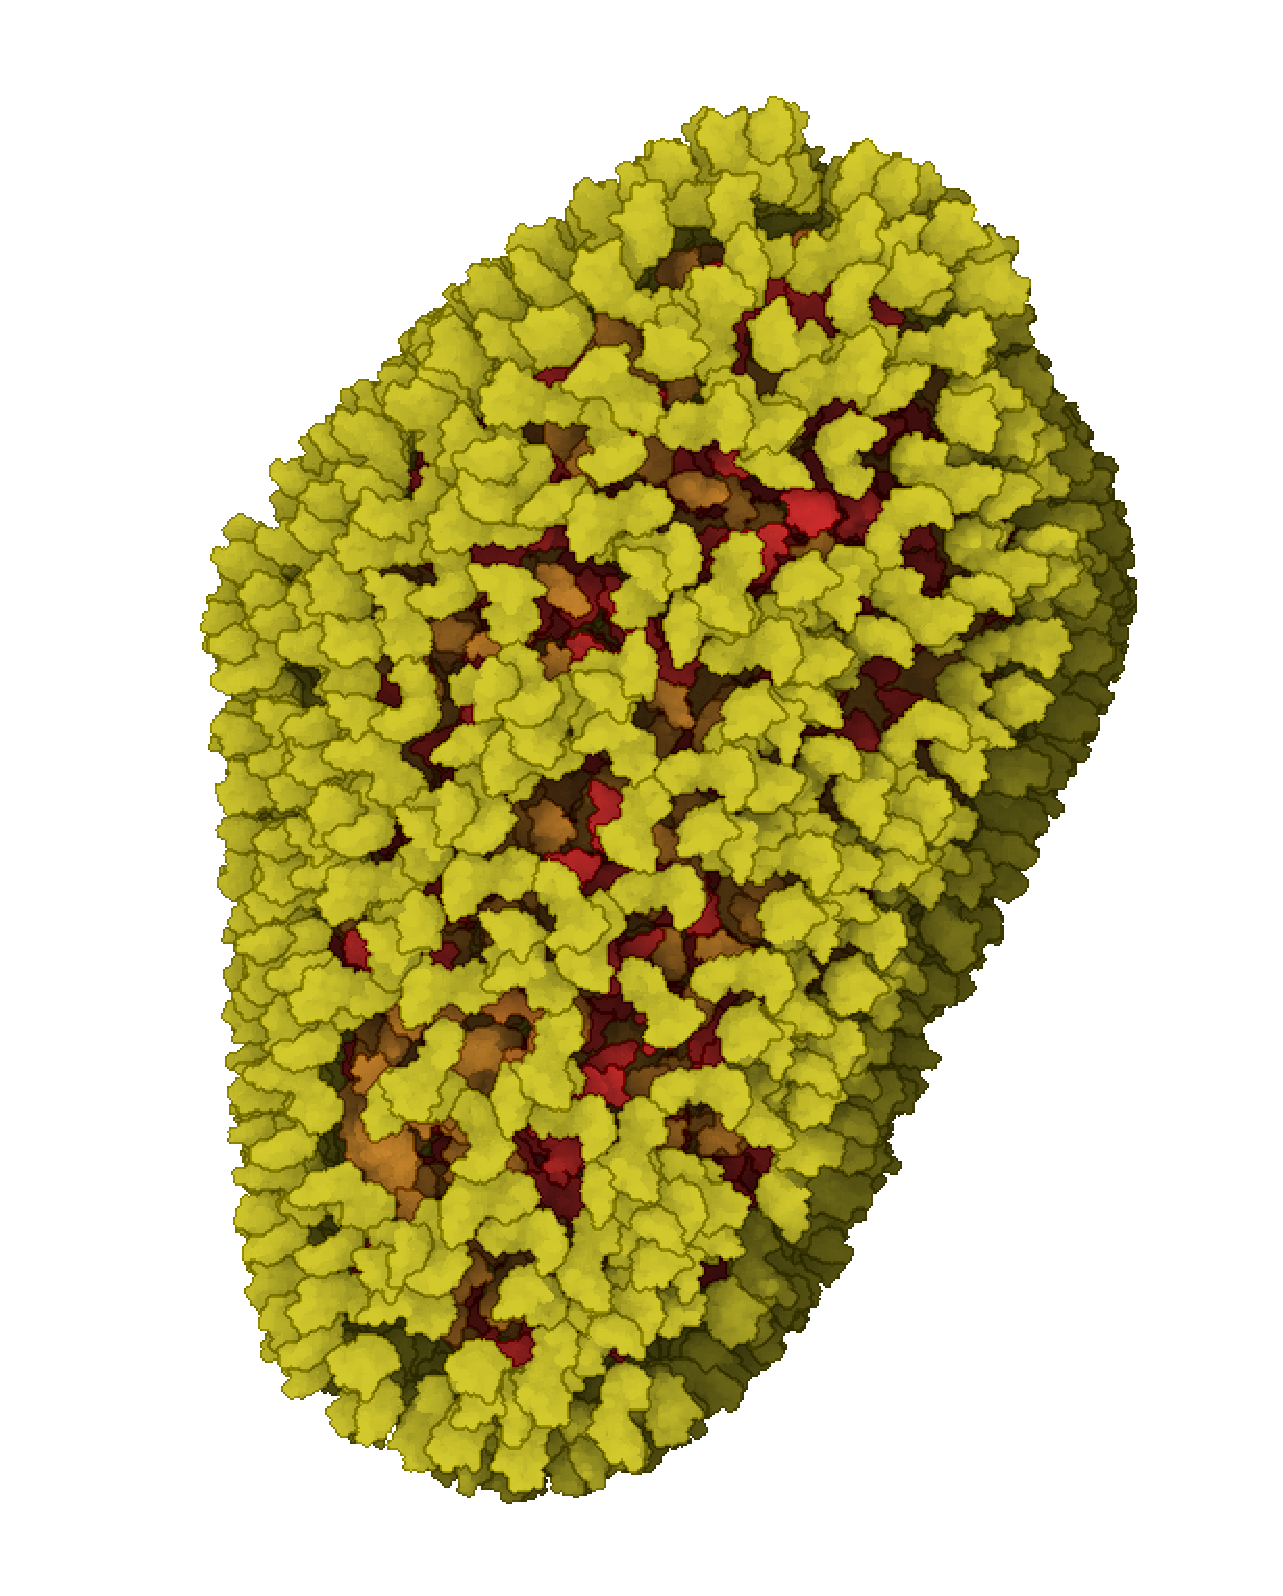
\includegraphics[width=0.25\linewidth]{figures/df1.eps}}
\subfloat[]{\label{fig:df2}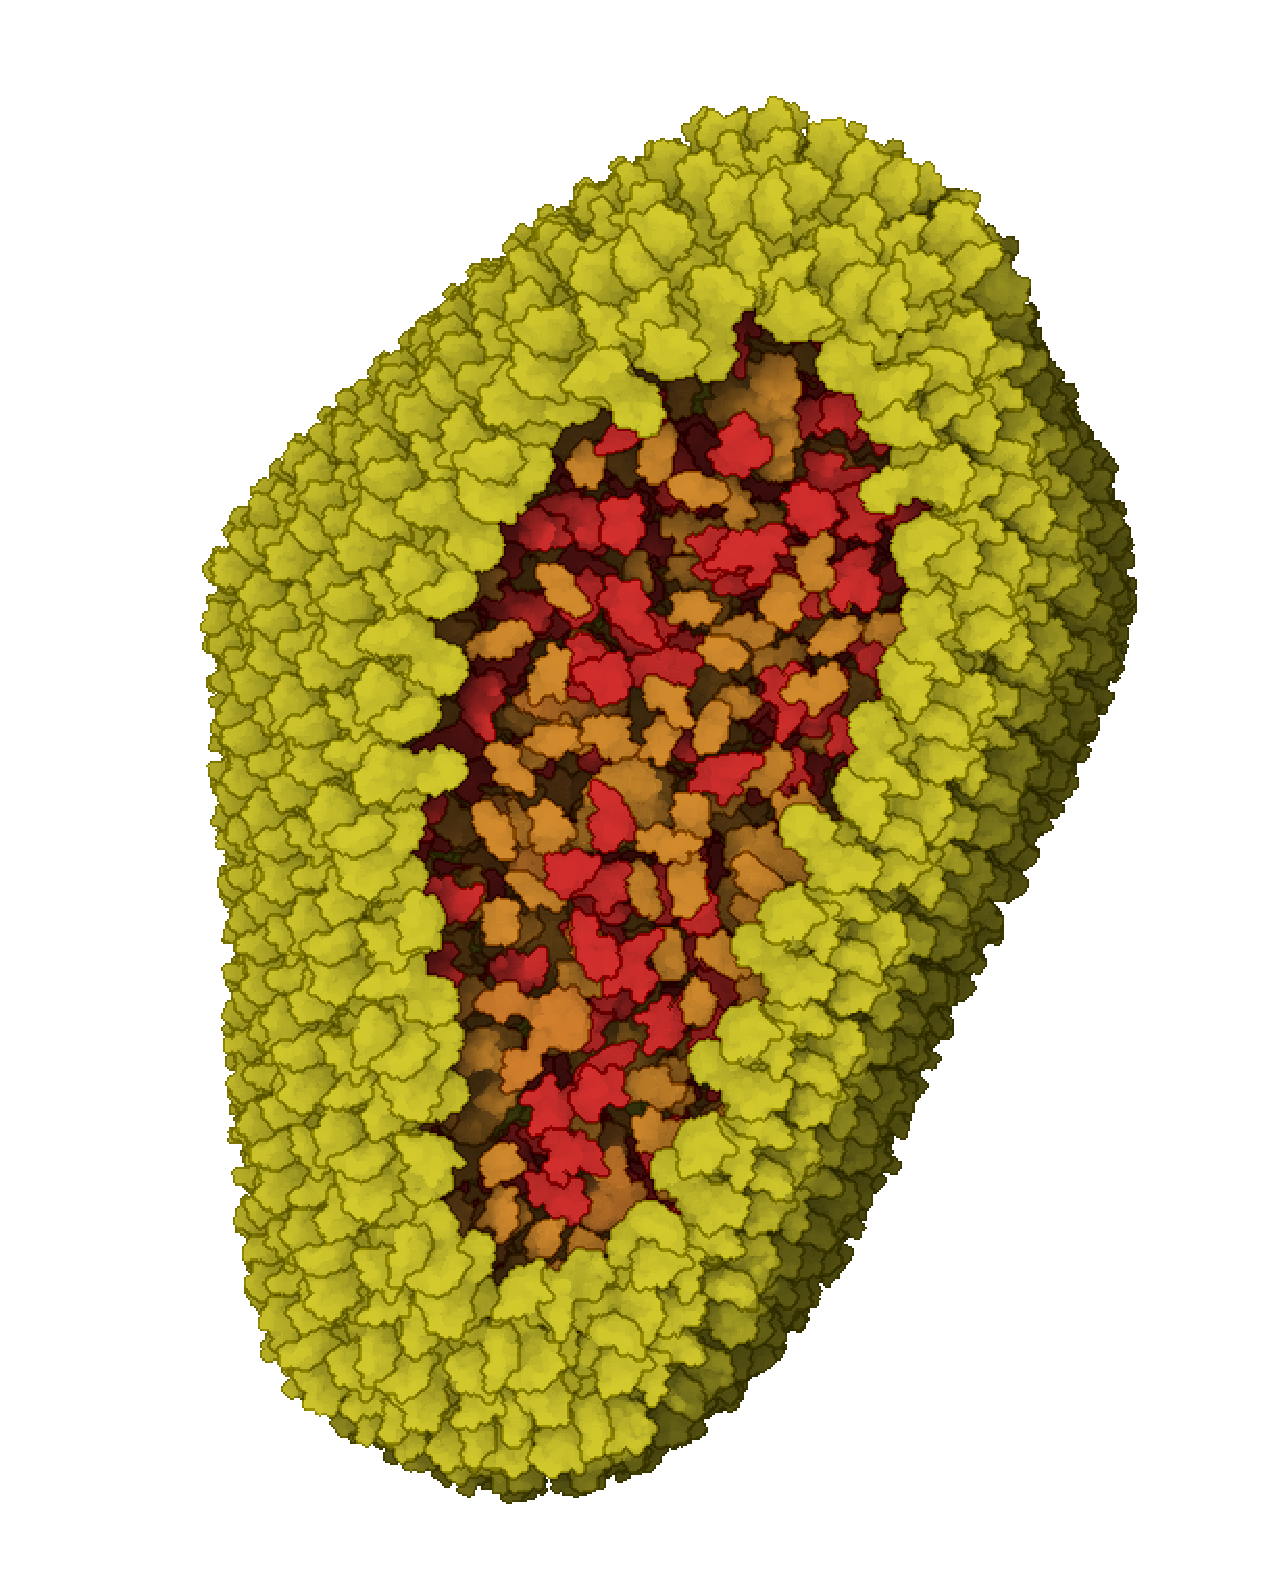
\includegraphics[width=0.25\linewidth]{figures/df2.eps}} 
\subfloat[]{\label{fig:df3}
\includegraphics[width=0.25\linewidth]{figures/df3.eps}}
\caption{\label{fig:df}View-space clipping, (a) shows the full HIV Capsid, (b) shows the uniformly distributed clipping, (c) demonstrate the aperture effect and (d) shows the results of the 2D distance transform of the clipping mask.}
\vspace{-2mm}
\end{figure}

\vspace{-2mm}
\section{View-Space Clipping}

While object space clipping with primitive shapes allows for a high degree of flexibility, it may also require cumbersome manual operations for more complex set-ups.
We therefore provide additional functionalities to selectively remove occluding instances in front of a set of ingredients set focus, to ensure them a maximum degree of visibility.
The focus state can be manually specified via the visibility equalizer by ticking a dedicated checkbox in front of the stack bars.
%We use occlusion queries to determine the instances located in front of the focus region. 
%We provide users with the option to control the degree of fuzziness of the clipping, similarly to object-space clipping.
%We also introduce a new effect inspired from the work of scientific illustrators, that allows users to control the degree of aperture of the view-space clipping.
%Finally, we modify our occlusion query method to improve depth perception. This is done by performing contextual anchoring which means that instances that would normally be clipped are kept when located in close vicinity to the focus region.

\vspace{-2mm}
\subsection{Occlusion Queries}
\label{sec:OQ}
%Focus ingredients are priorly selected from the user interface.
%In order to clip instances that are occluding the focus region, the most optimum approach in terms of efficiency and ease of implementation is without a doubt image-based.
%Modern graphics hardware already a fixed function called occlusion queries (OQ) and which allow to determine whether an instance is visible or hidden according to previously drawn geometries.
%This approach, however, would require issuing one draw call per queries, which can seriously effect the frame rate when issuing hundred of thousands of queries, because of GPU driver overhead.
%The rendering tool we are using already allows to render the entire scene in a single call to avoid latency due to the GPU driver.
%Due to the potentially large number of instances in the scenes we showcase, we accelerate the computation of occluding instances using an image-based approach on the GPU.
%However, for the sake of simplicity, we decide to assign only one occlusion mask per clipping object.
%, however, only one mask texture can be generated per clipping object.
%To achieve zero GPU driver overhead, we perform custom occlusion queries in a single draw call, using the programmable graphics pipeline.
%Subsequently, we draw the bounding sphere of all remaining instances over the mask.
%Due to early depth-stencil test, implicitly performed by the graphics hardware, 

When an ingredient type is set as focus, occluding instances of a different type may be selectively removed to reveal the occludees.
To determine which are the occluding instances, we perform occlusion queries. 
Nowadays, modern graphics hardware is able to perform occlusion queries easily using the fixed-functionality.
This method requires one draw call per query, which may induce driver overhead with several thousands of queries.
We compute the queries manually instead using a custom shader program, because it allows the queries to be computed in a single GPU draw call, thus approaching zero driver overhead.
Technical details about the approach are given by Kubisch \& Tavenrath \cite{kubisch2014opengl}.

We first render all the focused ingredients to an off-screen texture. 
The texture will then serve as a depth-stencil mask for the occlusion queries.
There can be several ingredient types constituting the object of focus for a given clipping object.
We render the bounding spheres of the potential occluders in a single draw call using instancing, on top of the depth-stencil mask.
Thanks to \emph{early depth-stencil} functionality available on modern graphics hardware, fragments that pass the test and be executed are guaranteed to belong to an occluder.
We then update the clipping state of the occluding instance by updating its corresponding occlusion flag stored in the GPU memory directly from the fragment \mbox{program}.

%An example of how we perform occlusion queries is shown in Figure \ref{fig:df0}.

\vspace{-2mm}
\subsection{Clipping Filtering}

Similarly to the object space clipping, we provide an additional parameter to control the degree of fuzziness of the view-dependent clipping, which we refer to as \emph{view-space clipping probability}.
This value is set by the user for each ingredient type, and is modified by dragging the dark green bar in the visibility equalizer.
The view-space clipping probability is evaluated after an instance was flagged as occluder in the same shader program mentioned in Section \ref{sec:OQ}.
We compare the clipping probability with a random number, initially defined and described in Section \ref{ssec:clip_params}.
If the random number is higher than the clipping probability, the instance will remain as clipped, otherwise it will be displayed. 
This will however result in a uniformly distributed number of visible occluders over the object of focus. 
Such a distribution might not always be the best design choice, because it fragments heavily the overall structure of the occluders and makes it difficult to see the occludees, as shown in Figure \ref{fig:df1}.

We propose an alternative technique for fuzzy removal of occluding instances, which we dub \emph{aperture effect}.
We define an additional parameter, the aperture coefficient, which controls the 2D distance from the instance to the edges of the occludees mask below which occluding instances shall be clipped.
A visual explanation of the aperture effect is shown in Figure \ref{fig:df2}.
To enable this effect we compute the 2D distance transform of the occludees mask which we store in a separate off-line texture.
We use the GPU Jump Flooding Algorithm by Rong \& Tan \cite{Rong06} to interactively recompute the 2D distance field every frame. 
After the computation of the distance transform, the texture stores the distance to the contours of the shape for each pixel.
Then, while computing occlusion queries in the fragment shader, we simply look-up the distance for the current fragment, and discard instances according to the user-defined aperture coefficient.
%, priorly set of each ingredient type.



\begin{figure}[t]
\centering
\includegraphics[width=0.7\linewidth]{figures/__hiv.eps}
\caption{\label{fig:hiv-islands} 
Illustration of contextual anchoring with an HIV particle. 
Despite the cutaway, some of the glyco-proteins (in yellow) are displayed and their surrounding lipid molecules (green) is preserved as contextual information.}
\vspace{-2mm}
\end{figure}

\subsection{Contextual Anchoring}
\label{ssec:anchoring}

When observing still images of cut-away scenes, it might be challenging to perceive the depth of objects correctly, despite using lighting-based depth cues.
We propose an additional method for depth guidance, which we call \emph{contextual anchoring}.
The concept is to override the results of clipping, to preserve elements located in proximity to non-clipped elements, and that would normally be clipped.
%By introducing contextual anchoring, the viewer, will intuitively understand where instances are located.
This principle in shown in Figure \ref{fig:hiv-islands}, where we can observe parts of the green membrane anchored around channel molecules, and which indicate that they are located on the surface of the object.
We were able to procedurally reproduce this effect by applying a depth bias to the occlusion queries computation for selected focused molecules.
This bias will ensure that contextual elements will no longer overlap the focus and will therefore be preserve as illustrated in Figure \ref{fig:islands}.



\begin{figure}[t]
\centering
\subfloat[]{\label{fig:df0}\includegraphics[width=0.45\linewidth]{figures/__islands-no.eps}}
\subfloat[]{\label{fig:islands1}\includegraphics[width=0.45\linewidth]{figures/__islands-yes.eps}}
\caption{\label{fig:islands} 
The principle of the depth-bias used for contextual anchoring.
The dark bars represents the depth values of the mask from the side, in one dimension. 
Elements in grey correspond to potentional occluders, while elements in red and green correspond to occludees.
The red type is subject to contextual anchoring.
(a) Without contextual anchoring, the depth of occluders (grey) is overlapping the depth of the mask and will therefore be discarded. 
(b) With contextual anchoring, the depth of the occludees (red) is shifted so that context elements (purple) no longer overlap the focus and remain unclipped.}
\vspace{-3mm}
\end{figure}

\section{Equalizing Visibility}



%The first section of the histogram (dark green region) shows the percentage of instances that are currently visible on the screen. 
%The entire green section (dark \& light green) represents the percentage of instances that are actually rendered.
%To provide a clear overview of the scene properties, we display stack bars for each ingredient type that indicate information about their degree of visibility.

The visibility equalizer comprises a series of stack bars that convey important visibility information for each ingredient type.
The three colors correspond respectively to the number of visible, occluded and clipped instances, as explained in Figure \ref{fig:ohist}.
In order to fill the stacked bars with correct values, we must count the number of clipped and visible instances, and this operation must be repeated on every update.

\vspace{-2mm}
\subsection{Counting Clipped Instances}

We perform the counting of the clipped instances on the GPU, in a dedicated compute shader program, since all the data already reside in the video memory.
We priorly declare a dedicated buffer on the GPU to hold the number of clipped instances for each ingredient type, and which shall be cleared before each counting operation.
Counting the clipped instances is a rather straightforward task since the clipping state of each instance is routinely computed and stored in a dedicated GPU buffer.
Once the clipping routine is performed, we simply browse through all the instances, and in case an instance was flagged as clipped, we increase the counter in the GPU buffer that corresponds to the number of clipped instances for the given type.
It is important to use an atomic increment operation for the counting to avoid concurrent accesses to the same counter value from different threads. 

\subsection{Counting Visible Instances}

In order to count the number of visible instances for a given view-point, we first need to generate an instance-buffer, which is a texture that contains, for each pixel, the unique instance id of the rendered molecule.
We first start to flag visible instances in a post-processing shader, by browsing all the pixels of the instance-buffer.
In case an instance is present in the instance-buffer, it is guaranteed to have at least one pixel visible on the screen, and it is therefore flagged as visible in a dedicated GPU buffer.
To store the number of visible instances per type, we also need to declare an additional GPU buffer, which must be priorly cleared each time visible instances are counted.
In a second stage, similarly to the counting of the clipped instances, we browse through all the instances in a dedicated compute shader, while fetching the visibility information which was previously computed.
Should an instance be flagged as visible, the counter that corresponds to the number of visible instances for the given type will be increase using an atomic increment operation.
Once the information about the number of visible and clipped instance is obtained, the data is then transferred to the CPU, and used to update the visibility equalizer.

\begin{comment}  

%\subsection{Visibility Tracking}

Modification of the visibility using the equalizer requires to know for each ingredient type, how many instances have been clipped and how many instances are actually visible on the screen, see Figure \ref{fig:ohist}.
Our system leverages the power of the GPU to compute the clipping state of each instance every frame.
Therefore, the information about clipping states is stored in the GPU memory.
In order to avoid an overhead due to data transfer between CPU and GPU, we perform the visibility tracking on the GPU using atomic operations.
%Atomic operations are parallel programming features which guarantee mutual exclusion when simultaneous thread wish to write in the same memory location.
We initially declare a buffer on the GPU to store the number of clipped and visible instances for each ingredient type.
To obtain the number of clipped instances, we simply increment the corresponding counter, each time an instance has been discarded using an atomic addition function.

For computing the number of visible instances, we first need information about actual visibility of rendered instances.
We render an additional off-screen texture where each pixel contains the internal ID of the instances.
We also declare an additional buffer to store a flag for each instance, which indicates if an instance is visible or hidden.
Then, by browsing through each pixel of the aforementioned ID texture in an additional pass, we update the visibility flag for the ID contained in each pixel.
Finally, we browse through each instance, and increment the corresponding counter according to the visibility flag using an atomic addition function, similar to the counting of clipped instances.

\subsection{User Interaction}

Upon interaction with the visibility equalizer, the system will either increase or decrease the number of clipped instances that correspond to the respective ingredient type.
This is intended to optimise the way users interact with the system, by offering a way to directly manipulate quantities rather than abstract internal values such as the clipping probability.
Additionally, the user may also manipulate more advanced parameters in an additional UI panel.
%We chose to map the motion of the histogram handles the clip probabilities.
%The first handle manipulates the view-space clipping probability, while the second handle controls the object-space one.
The clipping probabilities that are manipulated by the user correspond to the currently selected clipping object.
The displayed visibility in the equalizer, however, is valid for the entire scene.

%Quantities are relative by default, i.e, they represent a percentage of the total number of instances for a given ingredient.
%However, thanks to our design choices, they can also
Quantities shown in the visibility equalizer are ratios, not the absolute amounts. However, they can also be displayed as absolute quantities with limited additional effort.
For displaying absolute quantities, we support logarithmic scaling to ensure ingredients present in low quantities are visible in the stacked bars.
A logarithmic ruler is also provided to help the understanding of the displayed values.

\end{comment}  

%\section{Enhancements}

%Additionally to standard clipping functionality we developed a few enhancements to improve the way we perceive the scene.

%A crucial element when dealing with cluttered scenes is depth perception.

%Depth cues can be implemented by imitating the way light interact in reality to help us understanding distances between objects.

%However simulation illumination is rather expensive and prohibits a responsive user experience.

%We implement simplistic depth cues instead with a rough approximation of light behaviour.

%Additionally when provide option for context preserving view-space cut for a better understanding of the distance between objects in the view direction.

%Finally we perform rendering of the clipped element as ghosts in order to better communicate the overall proportions of visible elements in the scene.

%\subsection{Depth Cues}

%Depth cues are essential in molecular visualization and there exists many reference in the literature on how improve depth perception for that specific case.

%The first depth cue that we support is screen space ambient occlusion (SSAO) which allows to mimicate how global illumination works on the local scale, in image-space by evaluating for each pixel the depth of the surrounding pixels.

%Similarly to \cite{keylist}, we support two levels of ambient occlusion with different search radius to provide illumination for different levels of magnification.

%In addition to the limited range of the effect, SSAO does not account for directional light effects, which mean that shadows cannot be casted side-ways.

%When performing cut away however we perform strong shape alteration of the dataset which might be hard to perceive without shadows.

%Therefore, we additionally provide shadow mapping to better communicate the overall shape of the cuts.

%A downside of this approach is that it require an additional draw pass for each light that casts shadows onto molecules.

%Alternatively we also provide a cheaper method to provide additional cues about the shape of the clip objects.

%\textbf{TODO: PMINDEK, provide details about cheap depth cues}

%\subsection{Clipping Ghosts}

%While histograms allow us to visually monitor the quantities of removed instances, it might still be interesting to convey this information in the 3D scene while preserving  visibility settings.

%We additionally provide the option to render ghosts of all the clipped instances on top the scene, using alpha blending.

%We render all the ghosts in a separate off-screen texture which we later blend with the results of the scene rendering.

%The blending of the scene with the ghost texture is designed to ensure that the depth of the ghosts texture will merge with the scene's depth, and thus, that occluded ghosts will not be visible in the final results.

%We offer two rendering style for the ghosts, coloured filled or contour only.

%For each ingredient type we offer the option to render ghosts or not via the user interface.

%The resulting render of a scene with clipping ghosts can be seen in figure XX.


\section{Results and Performance Analysis}

To showcase the capabilities of our method, we applied it to three different mesoscale molecular scenes. 
For the rendering, we used cellVIEW \cite{muzic15}, a tool designed to efficiently render large molecular scenes on the GPU and implemented with Unity3D. 
The different datasets have been generated by the domain experts with cellPACK \cite{cellpack}, a modeling tool for procedural generation of large biomolecular structures.
cellPACK summarizes and incorporates the most recent knowledge obtained from structural biology and system biology to generate comprehensive mesoscale models. 
Based on experimentally obtained data (such as proteins structure, concentration and spatial distribution), the tool is able to generate entire models of viruses and cells via a packing method based on collision constraints.

%The results of the packing with cellPACK is stored in a file and loaded in cellVIEW afterwards.  
%The file generated by cellPACK contains the description of the scene, namely, position, rotation and type of each individual instances.
%In order the load and display the scene, cellVIEW reads the instances information from the file and uploads it on the GPU memory thus allowing fast read accesses from the rendering pipeline.

\begin{figure*}[t]
\centering
\subfloat[]{\label{fig:res:gh3}\includegraphics[width=0.33\linewidth]{figures/res-gh3.eps}}
\subfloat[]{\label{fig:res:myco}\includegraphics[width=0.26\linewidth]{figures/mycoplasma.eps}}
\subfloat[]{\label{fig:res:eq}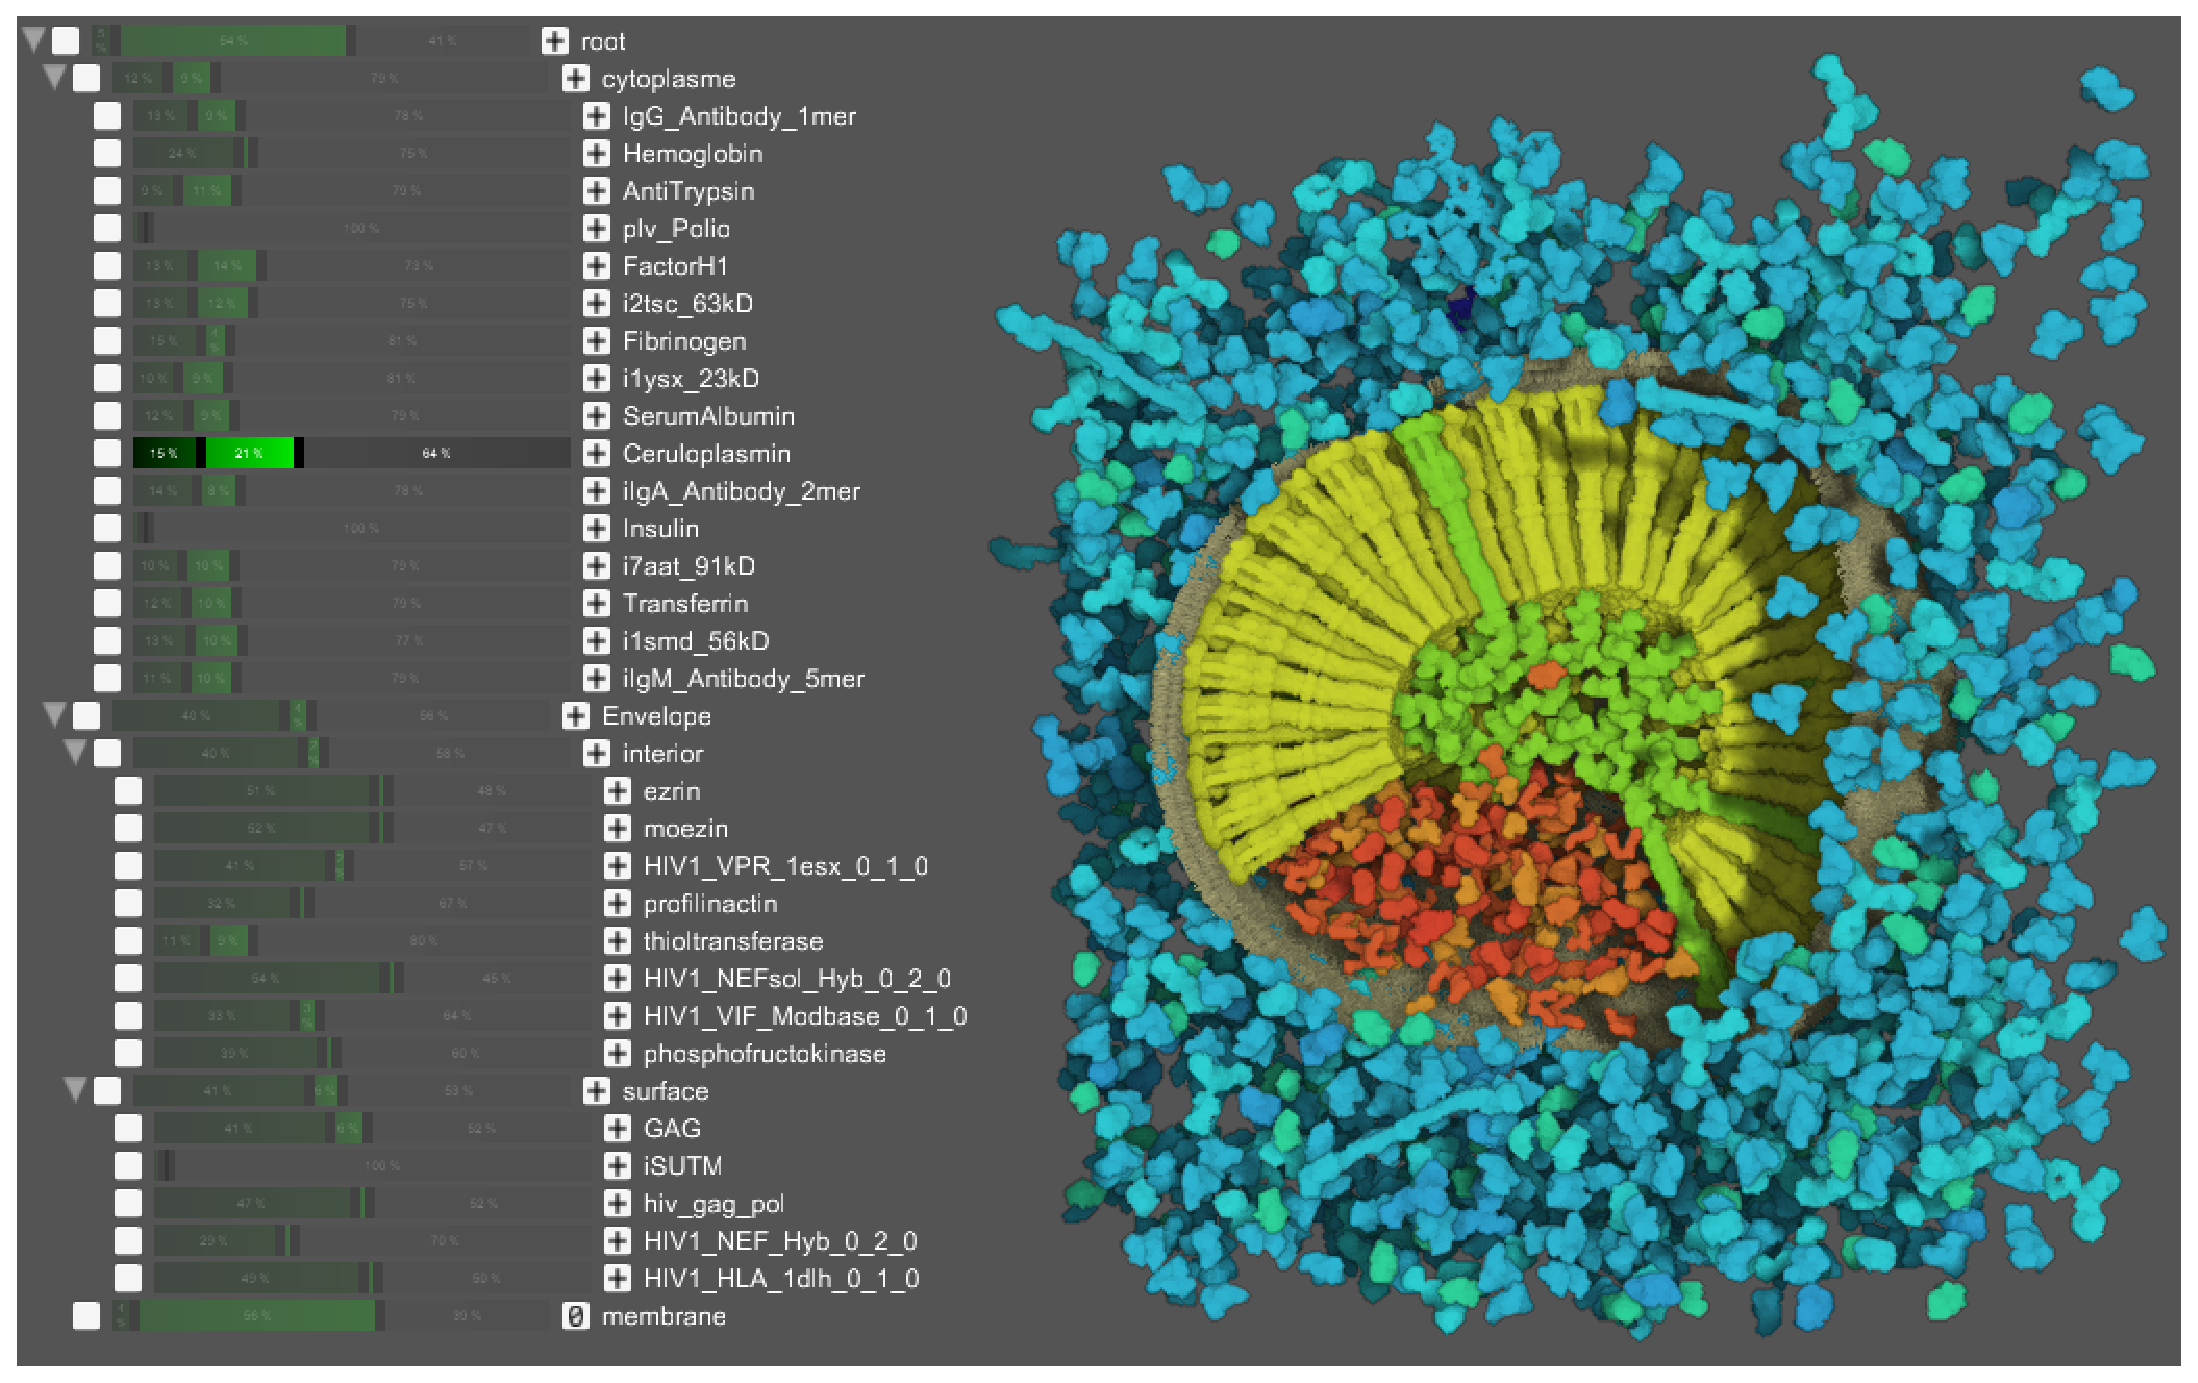
\includegraphics[width=0.4\linewidth]{figures/eq-s.eps}}
\caption{\label{fig:res:res}
Advanced clipping options in real test systems. (a) A falloff function is used to gradually clip serum molecules (red) from bottom to top to reveal the HIV capsid, with ghosting to give cues about the overall concentration. (b) Selective clipping is used to reveal the location of ribosome (blue) in a model of Mycoplasma mycoides.
(c) Internal structures of a immature HIV model are shown by several clipping objects. On the left, the visibility equalizer is shown.}
\vspace{-3mm}
\end{figure*}

The first dataset is a model of an HIV particle in blood serum that contains 20502 instances of 45 different protein types and 215559 instances of lipid molecules.
In Figure \ref{fig:res:gh3}, we show an example of a single clipping plane used to reduce the concentration of the blood serum molecules, so that the HIV proteins are visible. 
However, to avoid misleading the viewer about the actual concentration of the blood molecules, we render clipped proteins with a ghosting effect. 
This communicate true information about the concentration, while reducing visual clutter caused by the dense arrangement of blood serum proteins.
Figure \ref{fig:teaser} shows sequential step for production a comprehensible cut-away illustration with the HIV dataset.

The second dataset is a model of \emph{Mycoplasma mycoides} that contains 5380 proteins of 22 different types. 
Figure \ref{fig:res:myco} shows how fuzzy-clipping is used to reduce visual clutter to illustrate the positions of the ribosomes (shown in blue) within the cell.

The third dataset, shown in Figure \ref{fig:res:eq} is a model of an immature HIV which contains 1081 instances of 13 different protein types. 
We applied several clipping objects to reveal the internal structure of the virus. 
The blood serum (blue) has been preserved around the particle using the fuzzy clipping to illustrate how it encloses the HIV particle. 
The visibility equalizer is displayed as well, showing the ratios of visible and clipped instances of the individual molecular ingredients. 
The white boxes to the left of each stacked bar are used to mark the given ingredient or compartment as \mbox{focus}.

\begin{figure}[b]
\vspace{-4mm}
\centering
\includegraphics[width=0.89\linewidth]{figures/res-islands.eps}
\caption{\label{fig:res:islands}
HIV clipped with a plane. 
%Envelope proteins (blue) are reintroduced in the scene. 
Contextual anchoring is used to indicate the proximity of envelope proteins (dark blue) with the lipid membrane (grey)
The dark spots represent shadows projected into interior proteins.}
\end{figure}

Figure \ref{fig:res:islands} shows the mature HIV dataset clipped with a single plane. 
The contextual anchoring is applied to reintroduce parts of the clipped membrane (grey) around the envelope proteins (blue).

%\begin{figure}[t]
%\centering
%\subfloat[]{\label{fig:res:gh0}\includegraphics[width=0.5\linewidth]{figures/res-gh0.eps}}
%\subfloat[]{\label{fig:res:gh1}\includegraphics[width=0.5\linewidth]{figures/res-gh1.eps}}

%\subfloat[]{\label{fig:res:gh2}\includegraphics[width=0.5\linewidth]{figures/res-gh2.eps}}
%\subfloat[]{\label{fig:res:gh3}\includegraphics[width=0.5\linewidth]{figures/res-gh3.eps}}
%\caption{\label{fig:res:gh}The cutaway molecules are indicated through the ghosting effect. (a) Part of the scene is removed by a clipping plane. (b) The amount of cutaway molecules has been decreased through the fuzzy clipping, which caused some of the cutaway molecules to be reintroduced into the scene. (c) The blood serum (red molecules) are removed by fuzzy clipping in the entire dataset. (d) A falloff function is used to gradually change the influence of the fuzzy clipping.}
%\end{figure}
 
%Figure \ref{fig:res:gh} illustrates that this can be done in different ways according to the vision of the artist.

The visibility equalizer is designed to limit the computational overhead in order to offer a fast and responsive user experience.
To demonstrate the responsiveness of our method, we measured the computation time for the object-space clipping, view-space clipping and 2D distance transform, respectively.
The application was running on a machine equipped with an Intel Core i7-3930 CPU 3.20 GHz machine coupled with a GeForce GTX Titan X graphics card with 12GB of video RAM. 
The computation of the object-space clipping, compared to the rendering task performed by cellVIEW, is very lightweight and does not impact the overall performance too much. 
It took \textbf{0.3 milliseconds} to evaluate the 236061 instances of the HIV + blood dataset without clipping any of them.
It took \textbf{0.5 milliseconds} in total to slice the dataset in half and \textbf{0.6 milliseconds} to clip it entirely.
The increasing cost corresponds to the writing operations to the video memory, which are performed when an instance is clipped.
It is important to mention that neither the shape of the clipping object nor the number of clipping objects have a meaningful influence on the performance.

The view-space clipping, however, requires more computational work that could impact the responsiveness. 
%Therefore, a good strategy is to limit the number of view-space clipping objects, especially for very large scenes with up to several million instances. 
Indeed, for computing occlusion queries, occluders and occludees must be additionally rendered, which adds extra work to the rendering pipeline. 
For this reason, only the bounding spheres of the molecules are rendered instead of their entire structures, which may consist of hundreds or thousands of spheres, in order to guarantee a minimal computational overhead. 
We measured \textbf{0.07 milliseconds} for rendering the depth-stencil mask with 12142 instances (HIV proteins), and \textbf{0.57 milliseconds} for the computation of the 223919 occlusion queries corresponding to the remaining objects of the scene (blood proteins + lipid residues).
Additionally, the 2D distance transform that is needed for the aperture effect also requires additional computation.
It took \textbf{0.15 milliseconds} for computing the distance transform of the previous depth-stencil mask at a resolution of 512 by 512 pixels.
Unlike object-space clipping, the view-space clipping computation cost will keep increasing with additional operations.
Therefore it is a good strategy to keep a low number of view-space clipping objects, especially with very large scenes.

%\begin{figure}[t]
% \centering
%\includegraphics[width=\linewidth]{figures/eq-s.eps} %\caption{\label{fig:res:eq}Mature HIV.}
%\end{figure}


%\begin{figure}[t]
%\centering
%\subfloat[]{\label{fig:res:vsc0}\includegraphics[width=0.245\linewidth]{figures/res-vsc0.eps}}
%\hfill
%\subfloat[]{\label{fig:res:vsc1}\includegraphics[width=0.245\linewidth]{figures/res-vsc1.eps}}
%\hfill
%\subfloat[]{\label{fig:res:vsc2}\includegraphics[width=0.245\linewidth]{figures/res-vsc2.eps}}
%\hfill
%\subfloat[]{\label{fig:res:vsc3}\includegraphics[width=0.245\linewidth]{figures/res-vsc3.eps}}
%\caption{\label{fig:res:gh}View-space clipping.}
%\end{figure}

%\begin{figure*}[t]
%\centering

%\subfloat[]{\label{fig:res:w0}\includegraphics[width=0.25\linewidth]{figures/res-w0.eps}}
%\subfloat[]{\label{fig:res:w1}\includegraphics[width=0.25\linewidth]{figures/res-w1.eps}}
%\subfloat[]{\label{fig:res:w2}\includegraphics[width=0.25\linewidth]{figures/res-w2.eps}}
%\subfloat[]{\label{fig:res:w3}\includegraphics[width=0.25\linewidth]{figures/res-w3.eps}}

%\subfloat[]{\label{fig:res:w4}\includegraphics[width=0.25\linewidth]{figures/res-w4.eps}}
%\subfloat[]{\label{fig:res:w5}\includegraphics[width=0.25\linewidth]{figures/res-w5.eps}}
%\subfloat[]{\label{fig:res:w6}\includegraphics[width=0.25\linewidth]{figures/res-w6.eps}}
%\subfloat[]{\label{fig:res:w7}\includegraphics[width=0.25\linewidth]{figures/res-w7.eps}}
%\caption{\label{fig:res:w}W.}
%\end{figure*}

%\begin{figure}[t]
% \centering
% \includegraphics[width=\linewidth]{figures/results01.eps}
% \caption{\label{fig:results01}An illustration of the HIV virus in the %blood serum utilizing cutaways created with our approach.}
%\end{figure}


\section{User Feedback}
%Our visualization technique have the versatility to be useful for both, scientific exploration of large bio-molecular scene, and educational purposes.
%Our technique has potential for assisting scientific exploration of large molecular scenes, but it also has potential for educational purposes.

We evaluated the usefulness of our tool by collecting informal user feedback from domain experts in biological illustration and molecular biology.
In both cases, we did a remote walk-through introduction of our software, while collecting first impressions.
Additionally, we gave them an executable version of the software and asked them to write a short summary of their experience after trying the tool by themselves.
We first sent an early version of our tool to a biomedical illustrator with a strong academic background in chemistry. 
%He has 10 years of experience in the field of computer graphics and teaches online animation courses at CgSociety, with a focus on the creation of accurate biomolecular representations.
%He further gave computer graphics courses at his own institute (National research council of Italy), focusing on teaching basic skills in lighting and rendering to computer graphic novices.
His overall feedback was very positive, he enjoyed the responsiveness of the tool, and the novel concept of fuzziness and gradient clipping.
Here is a quote from his written feedback:

%I was really impressed by the quality of the non photo realistic toon rendering that can be achieved.
%It makes  the user able to create rendering of very complex scenes in few seconds that can be exported and tweaked for the final look in a composite software making the preproduction of high quality static rendering very fast
%I've never seen so far software that was able to manage with such a huge number of molecules/atoms without crashing.

\textit{``...in my opinion it can be a very useful toolkit for an illustrator in the biomedical field...It also seems very promising for interactive teaching and also for animation purposes...
One very useful feature of the software is the possibility to ``cut'' planes of interest of a particular space, and keeping the information of all ``layers'' by creating a ``gradient'' of concentration of the ingredients of the displayed molecular recipe. 
A visualization that resembles an ``exploded model'' but for biological assembly and it can be achieved without manually selecting every instance you would like to hide.''}

%which would be cumbersome to achieve with the tools he currently uses.
%Further, he was impressed with the responsiveness of the interactions with the visibility equalizer and the clipping planes.
%As a negative point, he mentioned the lack of exporting capabilities to mainstream animation packages such as Maya or Cinema 4D.

Secondly, we interviewed an expert in the domain of molecular biology and visualization. 
%His research focuses on the development and application of computational technologies to study the structure and function of biological molecules.
%His area of interest ranges from the design of therapeutic agents for AIDS, cancer and heart disease, to the development of novel algorithmic visualization and human interface approaches for molecular biology. 
%In nearly thirty years of experience, he has also contributed to a great number of molecular animations and visualizations that have appeared in popular books, magazines, newspapers and on television.
For this second interview, the overall feedback was also quite positive.
He greatly enjoyed how easy and fast it was to perform clipping, and also enjoyed the user interface for manipulating the cut object parameters.
He also wished for several additional features to improve the usability of the tool, such as filtering based on biomolecular properties and rendering the ghosts of the clipped instances.
These features have since been implemented in the current version of the software, as seen in Figure \ref{fig:res:gh3}.
Here is a quote from the written feedback we collected:

%This work provides a state-of-the-art and powerful interactive environment for visualizing and exploring  3D models of complex cellular environments with molecular detail. 
%Much of the problems in viewing and isolating various components of the model are assisted by the functions of this clipping environment. 
%Below are comments on some of the features and their utility

\textit{``...The aperture cutting feature is especially useful for exploring a feature or object in the context of a crowded molecular environment.
%The ability to shade the model with the aperture cut hightens the impression that the object being viewed is embedded in the volume.
%Without the shading, the object in the aperture appears to be floating above the surrounding environment when the model is interactively manipulated.
The ability to retain a subset of the clipped objects (``fuzzy clipping'') is an interesting feature that could be very useful under certain circumstances.
The feature is useful if one wants to get an impression of reducing the concentration of some of the molecular ingredients, or of what a gradient of certain molecular ingredients would look like.''}

%The approach would become even more useful if the selection of the unclipped objects could be based upon relationships between ingredients, such as retaining only selected molecules that are neighbors of one another.

%to improve how the tool could be employed more efficiently by his peers.
%The first wish was to add the possibility to filter molecules according to their biomolecular properties, such as the molecular weight or concentration.
%He also wished to see the ghosts of clipped instances in order to visually convey the proportions of removed elements in the 3D scene while preserving the current visibility setup.
%Additionally, he highly recommended us to add directional lighting to the scene in order to improve depth perception.

%To summarize, the evaluation showed that our equalizer-based approach for visibility specification was valuable and effective for both, scientific and educational purposes according to the opinion of domain experts.


\section{Conclusion and Future Work}

In this paper, we present a novel method for authoring cutaway illustrations of mesoscopic molecular models.
Our system uses clipping objects to selectively remove instances based on their type and location. 
To monitor and fine-tune the process, we introduce the visibility equalizer. 
It keeps the user informed about the number of molecular instances removed by the clipping objects, or occluded in the current viewport. 
Moreover, the visibility equalizer allows the users to directly override the behaviour of the clipping objects in order to fine-tune the visibility of molecular ingredients within the scene.

The visibility equalizer concept demonstrates a scenario where a visualization metaphor, such as the stacked bar chart, can serve as a user interface for performing a specific task, in our case to manipulate 3D data to authorize cutaways. 
The method allows users to create comprehensive illustrations of static biological models in realtime.
This was confirmed by gathering feedback from domain experts. 
While the concept was applied to a specific domain, we also wish to develop other examples where the (information) visualization would act simultaneously as an interface to steer the view.

There are also several follow-up ideas which we would like to focus on in the future, to strengthen data exploration and showcasing with cellVIEW.
Firstly, we would like to explore automatic clipping mechanisms to assist the user with the placement of clipping objects based on the nature of the scene and shape analysis.
Secondly, we would also like to try our visibility equalizer concept with time-dependent datasets and enhance it to provide the means for authoring illustrations of dynamic datasets.

Our Visibility Equalizer method is built on top of \mbox{cellVIEW} and Unity3D, which are both free to use for non-commercial use, the source code is publicly available, as well as the showcased scenes modelled with cellPACK (https://github.com/illvisation/cellVIEW).

 %, as well as by recreating existing illustrations with our method.
%While being simple to use, the method gives the user a considerable level of artistic freedom.
%The conceptual contribution of this work is demonstration of a scenario where a visualization metaphor, such as the stacked bar chart in our case, can serve as a user interface for performing a specific task, in our case authoring a cutaway design. 
%We expect to see further cases where the (information) visualization acts simultaneously as the user interface.
%During the whole authoring process, our method keeps the user informed about the ratios of the molecular instances removed by the clipping objects, or occluded from the current viewpoint. 

\section{Acknowledgement}

This project has been funded by the Vienna Science and Technology Fund (WWTF) through project VRG11-010 and also supported by EC Marie Curie Career Integration Grant through project PCIG13-GA-2013-618680. 
Autin,L. received support from the National Institutes of Health under award number P41GM103426. We would like to thank Aysylu Gabdulkhakova and Manuela Waldner for insightful comments.




%-------------------------------------------------------------------------

%\bibliographystyle{eg-alpha}
\bibliographystyle{eg-alpha-doi}

\bibliography{ref}

%-------------------------------------------------------------------------


\end{document}